\documentclass[]{article}
\usepackage{lmodern}
\usepackage{amssymb,amsmath}
\usepackage{ifxetex,ifluatex}
\usepackage{fixltx2e} % provides \textsubscript
\ifnum 0\ifxetex 1\fi\ifluatex 1\fi=0 % if pdftex
  \usepackage[T1]{fontenc}
  \usepackage[utf8]{inputenc}
\else % if luatex or xelatex
  \ifxetex
    \usepackage{mathspec}
    \usepackage{xltxtra,xunicode}
  \else
    \usepackage{fontspec}
  \fi
  \defaultfontfeatures{Mapping=tex-text,Scale=MatchLowercase}
  \newcommand{\euro}{€}
\fi
% use upquote if available, for straight quotes in verbatim environments
\IfFileExists{upquote.sty}{\usepackage{upquote}}{}
% use microtype if available
\IfFileExists{microtype.sty}{\usepackage{microtype}}{}
\usepackage[margin=1in]{geometry}
\usepackage{color}
\usepackage{fancyvrb}
\newcommand{\VerbBar}{|}
\newcommand{\VERB}{\Verb[commandchars=\\\{\}]}
\DefineVerbatimEnvironment{Highlighting}{Verbatim}{commandchars=\\\{\}}
% Add ',fontsize=\small' for more characters per line
\newenvironment{Shaded}{}{}
\newcommand{\AlertTok}[1]{\textcolor[rgb]{1.00,0.00,0.00}{\textbf{#1}}}
\newcommand{\AnnotationTok}[1]{\textcolor[rgb]{0.38,0.63,0.69}{\textbf{\textit{#1}}}}
\newcommand{\AttributeTok}[1]{\textcolor[rgb]{0.49,0.56,0.16}{#1}}
\newcommand{\BaseNTok}[1]{\textcolor[rgb]{0.25,0.63,0.44}{#1}}
\newcommand{\BuiltInTok}[1]{#1}
\newcommand{\CharTok}[1]{\textcolor[rgb]{0.25,0.44,0.63}{#1}}
\newcommand{\CommentTok}[1]{\textcolor[rgb]{0.38,0.63,0.69}{\textit{#1}}}
\newcommand{\CommentVarTok}[1]{\textcolor[rgb]{0.38,0.63,0.69}{\textbf{\textit{#1}}}}
\newcommand{\ConstantTok}[1]{\textcolor[rgb]{0.53,0.00,0.00}{#1}}
\newcommand{\ControlFlowTok}[1]{\textcolor[rgb]{0.00,0.44,0.13}{\textbf{#1}}}
\newcommand{\DataTypeTok}[1]{\textcolor[rgb]{0.56,0.13,0.00}{#1}}
\newcommand{\DecValTok}[1]{\textcolor[rgb]{0.25,0.63,0.44}{#1}}
\newcommand{\DocumentationTok}[1]{\textcolor[rgb]{0.73,0.13,0.13}{\textit{#1}}}
\newcommand{\ErrorTok}[1]{\textcolor[rgb]{1.00,0.00,0.00}{\textbf{#1}}}
\newcommand{\ExtensionTok}[1]{#1}
\newcommand{\FloatTok}[1]{\textcolor[rgb]{0.25,0.63,0.44}{#1}}
\newcommand{\FunctionTok}[1]{\textcolor[rgb]{0.02,0.16,0.49}{#1}}
\newcommand{\ImportTok}[1]{#1}
\newcommand{\InformationTok}[1]{\textcolor[rgb]{0.38,0.63,0.69}{\textbf{\textit{#1}}}}
\newcommand{\KeywordTok}[1]{\textcolor[rgb]{0.00,0.44,0.13}{\textbf{#1}}}
\newcommand{\NormalTok}[1]{#1}
\newcommand{\OperatorTok}[1]{\textcolor[rgb]{0.40,0.40,0.40}{#1}}
\newcommand{\OtherTok}[1]{\textcolor[rgb]{0.00,0.44,0.13}{#1}}
\newcommand{\PreprocessorTok}[1]{\textcolor[rgb]{0.74,0.48,0.00}{#1}}
\newcommand{\RegionMarkerTok}[1]{#1}
\newcommand{\SpecialCharTok}[1]{\textcolor[rgb]{0.25,0.44,0.63}{#1}}
\newcommand{\SpecialStringTok}[1]{\textcolor[rgb]{0.73,0.40,0.53}{#1}}
\newcommand{\StringTok}[1]{\textcolor[rgb]{0.25,0.44,0.63}{#1}}
\newcommand{\VariableTok}[1]{\textcolor[rgb]{0.10,0.09,0.49}{#1}}
\newcommand{\VerbatimStringTok}[1]{\textcolor[rgb]{0.25,0.44,0.63}{#1}}
\newcommand{\WarningTok}[1]{\textcolor[rgb]{0.38,0.63,0.69}{\textbf{\textit{#1}}}}
\usepackage{graphicx}
\makeatletter
\def\maxwidth{\ifdim\Gin@nat@width>\linewidth\linewidth\else\Gin@nat@width\fi}
\def\maxheight{\ifdim\Gin@nat@height>\textheight\textheight\else\Gin@nat@height\fi}
\makeatother
% Scale images if necessary, so that they will not overflow the page
% margins by default, and it is still possible to overwrite the defaults
% using explicit options in \includegraphics[width, height, ...]{}
\setkeys{Gin}{width=\maxwidth,height=\maxheight,keepaspectratio}
\ifxetex
  \usepackage[setpagesize=false, % page size defined by xetex
              unicode=false, % unicode breaks when used with xetex
              xetex]{hyperref}
\else
  \usepackage[unicode=true]{hyperref}
\fi
\hypersetup{breaklinks=true,
            bookmarks=true,
            pdfauthor={Justin Le},
            pdftitle={Hamiltonian Dynamics in Haskell},
            colorlinks=true,
            citecolor=blue,
            urlcolor=blue,
            linkcolor=magenta,
            pdfborder={0 0 0}}
\urlstyle{same}  % don't use monospace font for urls
% Make links footnotes instead of hotlinks:
\renewcommand{\href}[2]{#2\footnote{\url{#1}}}
\setlength{\parindent}{0pt}
\setlength{\parskip}{6pt plus 2pt minus 1pt}
\setlength{\emergencystretch}{3em}  % prevent overfull lines
\setcounter{secnumdepth}{0}

\title{Hamiltonian Dynamics in Haskell}
\author{Justin Le}
\date{November 27, 2017}

\begin{document}
\maketitle

\emph{Originally posted on
\textbf{\href{https://blog.jle.im/entry/hamiltonian-dynamics-in-haskell.html}{in
Code}}.}

As promised in my
\href{https://blog.jle.im/entry/introducing-the-hamilton-library.html}{\emph{hamilton}
introduction post} (published almost exactly one year ago!), I'm going to go
over implementing of the
\emph{\href{http://hackage.haskell.org/package/hamilton}{hamilton}} library
using

\begin{enumerate}
\def\labelenumi{\arabic{enumi}.}
\tightlist
\item
  \emph{DataKinds} (with \emph{TypeLits}) to enforce sizes of vectors and
  matrices and help guide us write our code
\item
  Statically-sized linear algebra with
  \emph{\href{http://hackage.haskell.org/package/hmatrix}{hmatrix}}
\item
  Automatic differentiation with
  \emph{\href{http://hackage.haskell.org/package/ad}{ad}}
\item
  Statically-sized vectors with
  \emph{\href{http://hackage.haskell.org/package/vector-sized}{vector-sized}}
\end{enumerate}

This post will be a bit heavy in some mathematics and Haskell concepts. The
expected audience is intermediate Haskell programmers. Note that this is
\emph{not} a post on dependent types, because dependent types (types that depend
on runtime values) are not explicitly used.

The mathematics and physics are ``extra'' flavor text and could potentially be
skipped, but you'll get the most out of this article if you have basic
familiarity with:

\begin{enumerate}
\def\labelenumi{\arabic{enumi}.}
\tightlist
\item
  Basic concepts of multivariable calculus (like partial and total derivatives).
\item
  Concepts of linear algebra (like dot products, matrix multiplication, and
  matrix inverses)
\end{enumerate}

No physics knowledge is assumed, but knowing a little bit of first semester
physics would help you gain a bit more of an appreciation for the end result!

The
\href{https://blog.jle.im/entry/introducing-the-hamilton-library.html}{hamilton
library introduction} should be considered a ``soft prerequisite'' for this
post, as it presents motivations, visual demonstrations, and general overviews
of the methods presented here!

\hypertarget{the-goal}{%
\section{The Goal}\label{the-goal}}

At the end of this, we should be able to have Haskell \emph{automatically
generate} \textbf{equations of motions} for any arbitrary system described in
arbitrary coordinate systems, and simulate that system.

Normally, we'd describe a system using particles' x and y coordinates, but our
goal is to be able to describe our particles' positions using any coordinate
system we want (polar, distance-along-a-curved-rail, pendulum-angles, etc.) and
have Haskell automatically generate equations of motions and time progressions
of those coordinates.

Read \href{https://blog.jle.im/entry/introducing-the-hamilton-library.html}{my
hamilton library introduction} for more information and examples!

\hypertarget{hamiltonian-mechanics}{%
\section{Hamiltonian Mechanics}\label{hamiltonian-mechanics}}

As mentioned in the previous post, Hamiltonian mechanics is a re-imagining of
dynamics and mechanics (think ``the world
post-\includegraphics{https://latex.codecogs.com/png.latex?F\%20\%3D\%20m\%20a}'')
that not only opened up new doors to solving problems in classical, but also
ended up being the right angle of viewing the world to unlock statistical
mechanics and thermodynamics, and later even quantum mechanics.

Hamiltonian mechanics lets you parameterize your system's ``position'' in
arbitrary ways (like the angle of rotation, for pendulum problems) and then
posits that the full state of the system exists in something called \emph{phase
space}, and that the system's dynamics is its motion through phase space that is
dictated by the geometry of the \emph{Hamiltonian} of that phase space.

The system's \emph{Hamiltonian} is a
\includegraphics{https://latex.codecogs.com/png.latex?\%5Cmathbb\%7BR\%7D\%5E\%7B2n\%7D\%20\%5Crightarrow\%20\%5Cmathbb\%7BR\%7D}
function from a point in
\includegraphics{https://latex.codecogs.com/png.latex?\%5Cmathbb\%7BR\%7D\%5E\%7B2n\%7D}
phase space (where \includegraphics{https://latex.codecogs.com/png.latex?n} is
the number of coordinates parameterizing your system) to a scalar in
\includegraphics{https://latex.codecogs.com/png.latex?\%5Cmathbb\%7BR\%7D}. For
a time-independent system, the picture of the dynamics is pretty simple: the
system moves along the \emph{contour lines} of the \emph{Hamiltonian} -- the
lines of equal ``height''.

\begin{figure}
\centering
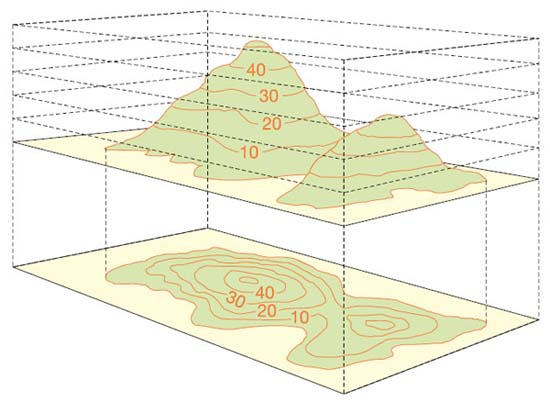
\includegraphics{/img/entries/hamilton/contour-lines.jpg}
\caption{Example of contour lines of a
\includegraphics{https://latex.codecogs.com/png.latex?\%5Cmathbb\%7BR\%7D\%5E2\%20\%5Crightarrow\%20\%5Cmathbb\%7BR\%7D}
function -- the elevation of land, from the
\href{https://www.ordnancesurvey.co.uk/blog/2015/11/map-reading-skills-making-sense-of-contour-lines/}{Ordinace
Survey} website.}
\end{figure}

In the example above, if we imagine that phase space is the 2D location, then
the \emph{Hamiltonian} is the mountain. And for a system dropped anywhere on the
mountain, its motion would be along the contour lines. For example, if a system
started somewhere along the 10 contour line, it would begin to oscillate the
entire phase space along the 10 contour line.\footnote{The picture with a
  time-dependent Hamiltonian is different, but only slightly. In the
  time-dependent case, the system still \emph{tries} to move along contour lines
  at every point in time, but the mountain is constantly changing underneath it
  and the contour lines keep on shifting underneath it. Sounds like life!}

\emph{Every} \href{https://www.youtube.com/watch?v=izGwDsrQ1eQ}{smooth}
\includegraphics{https://latex.codecogs.com/png.latex?\%5Cmathbb\%7BR\%7D\%5E\%7B2n\%7D\%20\%5Crightarrow\%20\%5Cmathbb\%7BR\%7D}
function on phase space can be used as a Hamiltonian to describe the physics of
some system. So, given any ``mountain range'' on phase space, any ``elevation
map'' or real-valued function on phase space, you can treat it as a description
of the dynamics of some physical system.

The \emph{trick}, then, to using Hamiltonian dynamics to model your system, is:

\begin{enumerate}
\def\labelenumi{\arabic{enumi}.}
\item
  Finding the phase space to describe your system. This can be done based on any
  continuous parameterization of your system (``generalized coordinates''), like
  angles of pendulums and so on.
\item
  Finding the Hamiltonian on that phase space to describe your system.
\end{enumerate}

And then Hamilton's dynamics will give you the rest! All you do is ``follow the
contour lines'' on that Hamiltonian!

\hypertarget{phase-space}{%
\subsection{Phase Space}\label{phase-space}}

Hamiltonian dynamics are about systems moving around in phase space. It seems
that phase space is the ``room where it happens'', so to speak, so let's dig
deeper into what it is. \emph{Phase space} is a
\includegraphics{https://latex.codecogs.com/png.latex?2n}-dimensional space
parameterized by:

\begin{enumerate}
\def\labelenumi{\arabic{enumi}.}
\tightlist
\item
  All of the current values of the
  \includegraphics{https://latex.codecogs.com/png.latex?n} parameters
  (``generalized coordinates'')
\item
  All of the current ``generalized momenta'' of those
  \includegraphics{https://latex.codecogs.com/png.latex?n} parameters
\end{enumerate}

So if you were parameterizing your pendulum system by, say, the angle of the
pendulum, then a point in phase space would be the current angle of the pendulum
along with the current ``generalized momentum'' associated with the angle of the
pendulum. What exactly \emph{is} generalized momentum? We'll go over calculating
it eventually, but what does it represent\ldots{}\emph{physically}?

The deeper answer involves the underlying Lie algebra of the Lie group
associated with the generalized coordinates, but going into that would make this
a completely different post. What I \emph{can} say is that the generalized
momenta associated with (``conjugate to'') certain sets of familiar coordinates
yield things that we typically call ``momenta'':

\begin{enumerate}
\def\labelenumi{\arabic{enumi}.}
\item
  The momentum conjugate to normal Cartesian coordinates is just our normal
  run-of-the-mill \emph{linear momentum} (in the
  \includegraphics{https://latex.codecogs.com/png.latex?\%5Cmathbf\%7Bp\%7D\%20\%3D\%20m\%20\%5Cmathbf\%7Bv\%7D})
  from first semester physics.
\item
  The momentum conjugate to the angle
  \includegraphics{https://latex.codecogs.com/png.latex?\%5Ctheta} in polar
  coordinates is \emph{angular momentum}
  (\includegraphics{https://latex.codecogs.com/png.latex?L\%20\%3D\%20m\%20r\%5E2\%20\%5Cdot\%7B\%5Ctheta\%7D})
  from first semester physics.
\item
  The momentum conjugate to the radial coordinate
  \includegraphics{https://latex.codecogs.com/png.latex?r} in polar coordinates
  is also just boring old linear momentum
  \includegraphics{https://latex.codecogs.com/png.latex?p_r\%20\%3D\%20m\%20\%5Cdot\%7Br\%7D},
  which makes sense because purely radial motion is just linear motion.
\end{enumerate}

So, it's our normal momentum (for linear and polar coordinates)
\emph{generalized} to arbitrary coordinates.

\hypertarget{hamiltonian-dynamics}{%
\subsection{Hamiltonian Dynamics}\label{hamiltonian-dynamics}}

I've explained Hamiltonian dynamics for time-independent Hamiltonians as
``follow the contour lines''. If you remember your basic multi-variable calculus
course, you'll know that the line of ``steepest ascent'' is the gradient. If we
call the Hamiltonian
\includegraphics{https://latex.codecogs.com/png.latex?\%5Cmathcal\%7BH\%7D\%28\%5Cmathbf\%7Bq\%7D\%2C\%5Cmathbf\%7Bp\%7D\%29}
(where
\includegraphics{https://latex.codecogs.com/png.latex?\%5Cmathbf\%7Bq\%7D} is
the vector of positions and
\includegraphics{https://latex.codecogs.com/png.latex?\%5Cmathbf\%7Bp\%7D} is
the vector of momenta), then the direction of steepest ascent is

{[} \textbackslash left \textbackslash langle
\textbackslash frac\{\textbackslash partial\}\{\textbackslash partial
\textbackslash mathbf\{q\}\}
\textbackslash mathcal\{H\}(\textbackslash mathbf\{q\},\textbackslash mathbf\{p\}),
\textbackslash frac\{\textbackslash partial\}\{\textbackslash partial
\textbackslash mathbf\{p\}\}
\textbackslash mathcal\{H\}(\textbackslash mathbf\{q\},\textbackslash mathbf\{p\})
\textbackslash right
\textbackslash rangle{]}(https://latex.codecogs.com/png.latex?\%0A\%5Cleft\%20\%5Clangle\%20\%5Cfrac\%7B\%5Cpartial\%7D\%7B\%5Cpartial\%20\%5Cmathbf\%7Bq\%7D\%7D\%0A\%5Cmathcal\%7BH\%7D\%28\%5Cmathbf\%7Bq\%7D\%2C\%5Cmathbf\%7Bp\%7D\%29\%2C\%20\%5Cfrac\%7B\%5Cpartial\%7D\%7B\%5Cpartial\%20\%5Cmathbf\%7Bp\%7D\%7D\%0A\%5Cmathcal\%7BH\%7D\%28\%5Cmathbf\%7Bq\%7D\%2C\%5Cmathbf\%7Bp\%7D\%29\%20\%5Cright\%20\%5Crangle\%0A
" \left \langle \frac{\partial}{\partial \mathbf{q}}
\mathcal{H}(\mathbf{q},\mathbf{p}), \frac{\partial}{\partial \mathbf{p}}
\mathcal{H}(\mathbf{q},\mathbf{p}) \right \rangle ")

But we want to move along the \emph{contour lines}\ldots and these are the lines
\emph{perpendicular} to the direction of steepest descent. The vector
perpendicular to
\includegraphics{https://latex.codecogs.com/png.latex?\%5Clangle\%20x\%2C\%20y\%20\%5Crangle}
is
\includegraphics{https://latex.codecogs.com/png.latex?\%5Clangle\%20y\%2C\%20-x\%20\%5Crangle},\footnote{There's
  also another perpendicular vector,
  \includegraphics{https://latex.codecogs.com/png.latex?\%5Clangle\%20-y\%2C\%20x\%20\%5Crangle},
  which actually gives motion \emph{backwards} in time.} so we just derived the
actual Hamiltonian equations of motion: just move in the direction perpendicular
to the steepest ascent! That is, to have things move on contour lines,
\includegraphics{https://latex.codecogs.com/png.latex?\%5Cdot\%7Bq\%7D} and
\includegraphics{https://latex.codecogs.com/png.latex?\%5Cdot\%7Bp\%7D_q}
\emph{should} be:

{[} \textbackslash begin\{aligned\} \textbackslash dot\{q\} \& =
\textbackslash frac\{\textbackslash partial\}\{\textbackslash partial p\_q\}
\textbackslash mathcal\{H\}(\textbackslash mathbf\{q\},\textbackslash mathbf\{p\})
\textbackslash\textbackslash{} \textbackslash dot\{p\}\_q \& = -
\textbackslash frac\{\textbackslash partial\}\{\textbackslash partial q\}
\textbackslash mathcal\{H\}(\textbackslash mathbf\{q\},\textbackslash mathbf\{p\})
\textbackslash end\{aligned\}{]}(https://latex.codecogs.com/png.latex?\%0A\%5Cbegin\%7Baligned\%7D\%0A\%5Cdot\%7Bq\%7D\%20\%26\%20\%3D\%20\%5Cfrac\%7B\%5Cpartial\%7D\%7B\%5Cpartial\%20p\_q\%7D\%20\%5Cmathcal\%7BH\%7D\%28\%5Cmathbf\%7Bq\%7D\%2C\%5Cmathbf\%7Bp\%7D\%29\%20\%5C\%5C\%0A\%5Cdot\%7Bp\%7D\_q\%20\%26\%20\%3D\%20-\%20\%5Cfrac\%7B\%5Cpartial\%7D\%7B\%5Cpartial\%20q\%7D\%20\%5Cmathcal\%7BH\%7D\%28\%5Cmathbf\%7Bq\%7D\%2C\%5Cmathbf\%7Bp\%7D\%29\%0A\%5Cend\%7Baligned\%7D\%0A
" \textbackslash begin\{aligned\} \dot{q} \& = \frac{\partial}{\partial p_q}
\mathcal{H}(\mathbf{q},\mathbf{p}) \textbackslash{} \dot{p}\_q \& = -
\frac{\partial}{\partial q} \mathcal{H}(\mathbf{q},\mathbf{p})
\textbackslash end\{aligned\} ")

This is a conclusion with one generalized coordinate
\includegraphics{https://latex.codecogs.com/png.latex?q}, but we can generalize
this to systems with multiple coordinates as well, as long as this holds for
\emph{every} \includegraphics{https://latex.codecogs.com/png.latex?q} and the
momentum conjugate to it
(\includegraphics{https://latex.codecogs.com/png.latex?p_q}). (For the rest of
this post,
\includegraphics{https://latex.codecogs.com/png.latex?\%5Cmathbf\%7Bq\%7D}
refers to the vector of coordinates,
\includegraphics{https://latex.codecogs.com/png.latex?q} refers to a single
specific coordinate, and
\includegraphics{https://latex.codecogs.com/png.latex?p_q} refers to the
momentum conjugate to that coordinate).

Essentially, these give you ``updating functions'' for
\includegraphics{https://latex.codecogs.com/png.latex?q} and
\includegraphics{https://latex.codecogs.com/png.latex?p_q} -- given
\includegraphics{https://latex.codecogs.com/png.latex?\%5Cmathcal\%7BH\%7D\%28\%5Cmathbf\%7Bq\%7D\%2C\%5Cmathbf\%7Bp\%7D\%29},
you have a way to ``update'' the particle's position in phase space. Just take
the partial derivatives of
\includegraphics{https://latex.codecogs.com/png.latex?\%5Cmathcal\%7BH\%7D} at
every step in time! To update
\includegraphics{https://latex.codecogs.com/png.latex?q}, nudge it by
\includegraphics{https://latex.codecogs.com/png.latex?\%5Cfrac\%7B\%5Cpartial\%7D\%7B\%5Cpartial\%20p_q\%7D\%20\%5Cmathcal\%7BH\%7D\%28\%5Cmathbf\%7Bq\%7D\%2C\%5Cmathbf\%7Bp\%7D\%29}.
To update \includegraphics{https://latex.codecogs.com/png.latex?p_q}, nudge it
by
\includegraphics{https://latex.codecogs.com/png.latex?-\%5Cfrac\%7B\%5Cpartial\%7D\%7B\%5Cpartial\%20q\%7D\%20\%5Cmathcal\%7BH\%7D\%28\%5Cmathbf\%7Bq\%7D\%2C\%5Cmathbf\%7Bp\%7D\%29}!

This picture is appealing to me in a visceral way because it sort of seems like
the system is ``surfing'' along the Hamiltonian's contour lines. It's being
``pushed'' \emph{faster} when the Hamiltonian is steeper, and slower when it's
more shallow. I can apply all my intuition as a surfer\footnote{Disclaimer: I am
  not a surfer.} to Hamiltonian mechanics!

\hypertarget{hamiltonian-dynamics-and-physical-systems}{%
\section{Hamiltonian Dynamics and Physical
Systems}\label{hamiltonian-dynamics-and-physical-systems}}

Earlier I mentioned that the two steps for applying Hamiltonian mechanics to
your system was figuring out your system's conjugate momenta and the appropriate
Hamiltonian. To explain this, I'm going to make a couple of simplifying
assumptions that make the job easier for the purposes of this article:

\begin{enumerate}
\def\labelenumi{\arabic{enumi}.}
\tightlist
\item
  Your coordinates and potential energy are time-independent.
\item
  Your potential energy function only depends on \emph{positions}, and not
  \emph{velocities}. (So nothing like friction or wind resistance or magnetic
  field vector potentials)
\end{enumerate}

With these assumptions, I'm going to skip over discussing the
\href{https://en.wikipedia.org/wiki/Lagrangian_mechanics}{Lagrangian} of the
system, which is the traditional way to do this. You can think of this section
as me presenting derived conclusions and skipping the derivations.

\hypertarget{conjugate-momenta}{%
\subsection{Conjugate Momenta}\label{conjugate-momenta}}

For systems with velocity-independent potential energies, it can be shown that
the momentum conjugate to coordinate
\includegraphics{https://latex.codecogs.com/png.latex?q} is

{[} p\_q = \textbackslash frac\{\textbackslash partial\}\{\textbackslash partial
\textbackslash dot\{q\}\} KE(\textbackslash mathbf\{q\},
\textbackslash dot\{\textbackslash mathbf\{q\}\}){]}(https://latex.codecogs.com/png.latex?\%0Ap\_q\%20\%3D\%20\%5Cfrac\%7B\%5Cpartial\%7D\%7B\%5Cpartial\%20\%5Cdot\%7Bq\%7D\%7D\%20KE\%28\%5Cmathbf\%7Bq\%7D\%2C\%20\%5Cdot\%7B\%5Cmathbf\%7Bq\%7D\%7D\%29\%0A
" p\_q = \frac{\partial}{\partial \dot{q}} KE(\mathbf{q}, \dot{\mathbf{q}}) ")

Where
\includegraphics{https://latex.codecogs.com/png.latex?KE\%28\%5Cmathbf\%7Bq\%7D\%2C\%5Cdot\%7B\%5Cmathbf\%7Bq\%7D\%7D\%29}
is the kinetic energy of the system, which is a function on the coordinates
\includegraphics{https://latex.codecogs.com/png.latex?\%5Cmathbf\%7Bq\%7D} and
their rates of change,
\includegraphics{https://latex.codecogs.com/png.latex?\%5Cdot\%7B\%5Cmathbf\%7Bq\%7D\%7D}.
For example, for normal Cartesian coordinates in one dimension,
\includegraphics{https://latex.codecogs.com/png.latex?KE\%28x\%2C\%20\%5Cdot\%7Bx\%7D\%29\%20\%3D\%20\%5Cfrac\%7B1\%7D\%7B2\%7D\%20m\%20\%5Cdot\%7Bx\%7D\%5E2}.
So the momentum conjugate to
\includegraphics{https://latex.codecogs.com/png.latex?x} is:

{[} p\_x = \textbackslash frac\{\textbackslash partial\}\{\textbackslash partial
\textbackslash dot\{x\}\} \textbackslash left{[} \textbackslash frac\{1\}\{2\} m
\textbackslash dot\{x\}\^{}2 \textbackslash right{]} = m
\textbackslash dot\{x\}{]}(https://latex.codecogs.com/png.latex?\%0Ap\_x\%20\%3D\%20\%5Cfrac\%7B\%5Cpartial\%7D\%7B\%5Cpartial\%20\%5Cdot\%7Bx\%7D\%7D\%20\%5Cleft\%5B\%20\%5Cfrac\%7B1\%7D\%7B2\%7D\%20m\%20\%5Cdot\%7Bx\%7D\%5E2\%20\%5Cright\%5D\%20\%3D\%20m\%20\%5Cdot\%7Bx\%7D\%0A
" p\_x = \frac{\partial}{\partial \dot{x}}
\left[ \frac{1}{2} m \dot{x}^2 \right] = m \dot{x} ")

Just linear momentum, like I claimed before.

Let's generalize this to arbitrary coordinates. In general, for \emph{Cartesian}
coordinates, the kinetic energy will always be

{[} KE(\textbackslash mathbf\{x\},
\textbackslash dot\{\textbackslash mathbf\{x\}\}) =
\textbackslash frac\{1\}\{2\} \textbackslash left{[} m\_1
\textbackslash dot\{x\}\_1\^{}2 + m\_2 \textbackslash dot\{x\}\_2\^{}2 + m\_3
\textbackslash dot\{x\}\_3\^{}2 + \textbackslash dots
\textbackslash right{]}{]}(https://latex.codecogs.com/png.latex?\%0AKE\%28\%5Cmathbf\%7Bx\%7D\%2C\%20\%5Cdot\%7B\%5Cmathbf\%7Bx\%7D\%7D\%29\%20\%3D\%20\%5Cfrac\%7B1\%7D\%7B2\%7D\%20\%5Cleft\%5B\%20m\_1\%20\%5Cdot\%7Bx\%7D\_1\%5E2\%20\%2B\%20m\_2\%20\%5Cdot\%7Bx\%7D\_2\%5E2\%20\%2B\%20m\_3\%20\%5Cdot\%7Bx\%7D\_3\%5E2\%20\%2B\%20\%5Cdots\%20\%5Cright\%5D\%0A
" KE(\mathbf{x}, \dot{\mathbf{x}}) = \frac{1}{2}
\left[ m_1 \dot{x}_1^2 + m_2 \dot{x}_2^2 + m_3 \dot{x}_3^2 + \dots \right]")

Where \includegraphics{https://latex.codecogs.com/png.latex?m} is the inertia
associated with each coordinate\ldots for example, if
\includegraphics{https://latex.codecogs.com/png.latex?\%5Clangle\%20x_1\%2C\%20x_2\%20\%5Crangle}
describes the location of an object of mass
\includegraphics{https://latex.codecogs.com/png.latex?m}, then
\includegraphics{https://latex.codecogs.com/png.latex?m_1\%20\%3D\%20m_2\%20\%3D\%20m}.

To give us nice notation and make things more convenient, we'll write this as a
quadratic form over an inertia matrix:

{[} KE(\textbackslash dot\{\textbackslash mathbf\{x\}\}) =
\textbackslash frac\{1\}\{2\}
\textbackslash dot\{\textbackslash mathbf\{x\}\}\^{}T \textbackslash hat\{M\}
\textbackslash dot\{\textbackslash mathbf\{x\}\}{]}(https://latex.codecogs.com/png.latex?\%0AKE\%28\%5Cdot\%7B\%5Cmathbf\%7Bx\%7D\%7D\%29\%20\%3D\%20\%5Cfrac\%7B1\%7D\%7B2\%7D\%20\%5Cdot\%7B\%5Cmathbf\%7Bx\%7D\%7D\%5ET\%20\%5Chat\%7BM\%7D\%20\%5Cdot\%7B\%5Cmathbf\%7Bx\%7D\%7D\%0A
" KE(\dot{\mathbf{x}}) = \frac{1}{2} \dot{\mathbf{x}}\^{}T \hat{M}
\dot{\mathbf{x}} ")

Where \includegraphics{https://latex.codecogs.com/png.latex?\%5Chat\%7BM\%7D} is
the \href{https://en.wikipedia.org/wiki/Diagonal_matrix}{diagonal matrix} whose
entries are the masses of each coordinate, and
\includegraphics{https://latex.codecogs.com/png.latex?\%5Cdot\%7B\%5Cmathbf\%7Bx\%7D\%7D}
is the column vector of all of the (Cartesian) coordinates,
\includegraphics{https://latex.codecogs.com/png.latex?\%5Cleft\%5B\%20\%5Cdot\%7Bx\%7D_1\%5C\%2C\%20\%5Cdot\%7Bx\%7D_2\%5C\%2C\%20\%5Cdot\%7Bx\%7D_3\%5C\%2C\%20\%5Cdots\%20\%5Cright\%5D\%5ET}.

Now! How to generalize this to arbitrary coordinates? Well, if we have
\includegraphics{https://latex.codecogs.com/png.latex?n} generalized coordinates
\includegraphics{https://latex.codecogs.com/png.latex?\%5Cmathbf\%7Bq\%7D}
mapping to \includegraphics{https://latex.codecogs.com/png.latex?m}-dimensional
Cartesian coordinates, we can specify them as
\includegraphics{https://latex.codecogs.com/png.latex?\%5Cmathbf\%7Bx\%7D\%20\%3D\%20f\%28\%5Cmathbf\%7Bq\%7D\%29},
where
\includegraphics{https://latex.codecogs.com/png.latex?f\%20\%3A\%20\%5Cmathbb\%7BR\%7D\%5En\%20\%5Crightarrow\%20\%5Cmathbb\%7BR\%7D\%5Em},
taking the vector of generalized coordinates and returning a vector for the
position in Cartesian space. For example, for polar coordinates,
\includegraphics{https://latex.codecogs.com/png.latex?f\%28r\%2C\%20\%5Ctheta\%29\%20\%3D\%20\%5Cleft\%20\%5Clangle\%20r\%20\%5Ccos\%28\%5Ctheta\%29\%2C\%20r\%20\%5Csin\%28\%5Ctheta\%29\%20\%5Cright\%20\%5Crangle},
because, for polar coordinates,
\includegraphics{https://latex.codecogs.com/png.latex?x\%20\%3D\%20r\%20\%5Ccos\%28\%5Ctheta\%29}
and
\includegraphics{https://latex.codecogs.com/png.latex?y\%20\%3D\%20r\%20\%5Csin\%28\%5Ctheta\%29}.

So we can get
\includegraphics{https://latex.codecogs.com/png.latex?\%5Cmathbf\%7Bx\%7D} from
\includegraphics{https://latex.codecogs.com/png.latex?\%5Cmathbf\%7Bq\%7D} with
\includegraphics{https://latex.codecogs.com/png.latex?f}, but how can we get
\includegraphics{https://latex.codecogs.com/png.latex?\%5Cdot\%7B\%5Cmathbf\%7Bx\%7D\%7D},
the vector of rate of changes? Well, if
\includegraphics{https://latex.codecogs.com/png.latex?x_1\%20\%3D\%20f_1\%28q_1\%2C\%20q_2\%2C\%20q_3\%20\%5Cdots\%29},
then the
\includegraphics{https://latex.codecogs.com/png.latex?\%5Cdot\%7Bx\%7D_1} is the
\href{https://en.wikipedia.org/wiki/Total_derivative}{total derivative} of
\includegraphics{https://latex.codecogs.com/png.latex?x_1} with respect to time:

{[} \textbackslash dot\{x\}\_1 = \textbackslash frac\{\textbackslash partial
f\_1\}\{\textbackslash partial q\_1\} \textbackslash dot\{q\}\_1 +
\textbackslash frac\{\textbackslash partial f\_1\}\{\textbackslash partial
q\_2\} \textbackslash dot\{q\}\_2 + \textbackslash frac\{\textbackslash partial
f\_1\}\{\textbackslash partial q\_3\} \textbackslash dot\{q\}\_3 +
\textbackslash dots{]}(https://latex.codecogs.com/png.latex?\%0A\%5Cdot\%7Bx\%7D\_1\%20\%3D\%20\%5Cfrac\%7B\%5Cpartial\%20f\_1\%7D\%7B\%5Cpartial\%20q\_1\%7D\%20\%5Cdot\%7Bq\%7D\_1\%20\%2B\%0A\%20\%20\%20\%20\%5Cfrac\%7B\%5Cpartial\%20f\_1\%7D\%7B\%5Cpartial\%20q\_2\%7D\%20\%5Cdot\%7Bq\%7D\_2\%20\%2B\%0A\%20\%20\%20\%20\%5Cfrac\%7B\%5Cpartial\%20f\_1\%7D\%7B\%5Cpartial\%20q\_3\%7D\%20\%5Cdot\%7Bq\%7D\_3\%20\%2B\%20\%5Cdots\%0A
" \dot{x}\_1 = \frac{\partial f_1}{\partial q_1} \dot{q}\_1 +
\frac{\partial f_1}{\partial q_2} \dot{q}\_2 + \frac{\partial f_1}{\partial q_3}
\dot{q}\_3 + \dots ")

Or, in short:

{[} \textbackslash dot\{x\}\_i = \textbackslash sum\_\{j = 1\}\^{}n
\textbackslash frac\{\textbackslash partial f\_i\}\{\textbackslash partial
q\_j\}
\textbackslash dot\{q\}\_j{]}(https://latex.codecogs.com/png.latex?\%0A\%5Cdot\%7Bx\%7D\_i\%20\%3D\%20\%5Csum\_\%7Bj\%20\%3D\%201\%7D\%5En\%20\%5Cfrac\%7B\%5Cpartial\%20f\_i\%7D\%7B\%5Cpartial\%20q\_j\%7D\%20\%5Cdot\%7Bq\%7D\_j\%0A
" \dot{x}\emph{i = \sum}\{j = 1\}\^{}n \frac{\partial f_i}{\partial q_j}
\dot{q}\_j ")

But, hey, this looks a lot like a matrix-vector multiplication! If we make
\includegraphics{https://latex.codecogs.com/png.latex?\%5Chat\%7BJ\%7D_f}, an
\includegraphics{https://latex.codecogs.com/png.latex?m\%20\%5Ctimes\%20n}
matrix of partial derivatives of
\includegraphics{https://latex.codecogs.com/png.latex?f}
(\includegraphics{https://latex.codecogs.com/png.latex?\%5Chat\%7BJ\%7D_\%7Bfij\%7D\%20\%3D\%20\%5Cfrac\%7B\%5Cpartial\%20f_i\%7D\%7B\%5Cpartial\%20q_j\%7D})
at a given point (typically called the
\href{https://en.wikipedia.org/wiki/Jacobian_matrix_and_determinant}{Jacobian
matrix of f}, then we have a nice expression for
\includegraphics{https://latex.codecogs.com/png.latex?\%5Cdot\%7B\%5Cmathbf\%7Bx\%7D\%7D}:

{[} \textbackslash dot\{\textbackslash mathbf\{x\}\} =
\textbackslash hat\{J\}\_f
\textbackslash dot\{\textbackslash mathbf\{q\}\}{]}(https://latex.codecogs.com/png.latex?\%0A\%5Cdot\%7B\%5Cmathbf\%7Bx\%7D\%7D\%20\%3D\%20\%5Chat\%7BJ\%7D\_f\%20\%5Cdot\%7B\%5Cmathbf\%7Bq\%7D\%7D\%0A
" \dot{\mathbf{x}} = \hat{J}\_f \dot{\mathbf{q}} ")

And we can plug it in (remembering that
\includegraphics{https://latex.codecogs.com/png.latex?\%28A\%20B\%29\%5ET\%20\%3D\%20B\%5ET\%20A\%5ET})
to our kinetic energy equation to get:

{[}
KE(\textbackslash mathbf\{q\},\textbackslash dot\{\textbackslash mathbf\{q\}\})
= \textbackslash frac\{1\}\{2\}
\textbackslash dot\{\textbackslash mathbf\{q\}\}\^{}T
\textbackslash hat\{J\}\_f\^{}T \textbackslash hat\{M\}
\textbackslash hat\{J\}\_f
\textbackslash dot\{\textbackslash mathbf\{q\}\}{]}(https://latex.codecogs.com/png.latex?\%0AKE\%28\%5Cmathbf\%7Bq\%7D\%2C\%5Cdot\%7B\%5Cmathbf\%7Bq\%7D\%7D\%29\%20\%3D\%20\%5Cfrac\%7B1\%7D\%7B2\%7D\%20\%5Cdot\%7B\%5Cmathbf\%7Bq\%7D\%7D\%5ET\%20\%5Chat\%7BJ\%7D\_f\%5ET\%0A\%20\%20\%20\%20\%5Chat\%7BM\%7D\%20\%5Chat\%7BJ\%7D\_f\%20\%5Cdot\%7B\%5Cmathbf\%7Bq\%7D\%7D\%0A
" KE(\mathbf{q},\dot{\mathbf{q}}) = \frac{1}{2} \dot{\mathbf{q}}\^{}T
\hat{J}\_f\^{}T \hat{M} \hat{J}\_f \dot{\mathbf{q}} ")

And for the final step, we differentiate with respect to the
\includegraphics{https://latex.codecogs.com/png.latex?\%5Cdot\%7Bq\%7D}s (which
is just the gradient
\includegraphics{https://latex.codecogs.com/png.latex?\%5Cnabla_\%7B\%5Cdot\%7B\%5Cmathbf\%7Bq\%7D\%7D\%7D})
to get
\includegraphics{https://latex.codecogs.com/png.latex?\%5Cmathbf\%7Bp\%7D}, the
vector of conjugate momenta:

{[} \textbackslash mathbf\{p\} =
\textbackslash nabla\_\{\textbackslash dot\{\textbackslash mathbf\{q\}\}\}
\textbackslash left{[} \textbackslash frac\{1\}\{2\}
\textbackslash dot\{\textbackslash mathbf\{q\}\}\^{}T
\textbackslash hat\{J\}\_f\^{}T \textbackslash hat\{M\}
\textbackslash hat\{J\}\_f \textbackslash dot\{\textbackslash mathbf\{q\}\}
\textbackslash right{]} = \textbackslash hat\{J\}\_f\^{}T
\textbackslash hat\{M\} \textbackslash hat\{J\}\_f
\textbackslash dot\{\textbackslash mathbf\{q\}\}{]}(https://latex.codecogs.com/png.latex?\%0A\%5Cmathbf\%7Bp\%7D\%20\%3D\%20\%5Cnabla\_\%7B\%5Cdot\%7B\%5Cmathbf\%7Bq\%7D\%7D\%7D\%20\%5Cleft\%5B\%0A\%20\%20\%20\%20\%5Cfrac\%7B1\%7D\%7B2\%7D\%20\%5Cdot\%7B\%5Cmathbf\%7Bq\%7D\%7D\%5ET\%20\%5Chat\%7BJ\%7D\_f\%5ET\%20\%5Chat\%7BM\%7D\%20\%5Chat\%7BJ\%7D\_f\%20\%5Cdot\%7B\%5Cmathbf\%7Bq\%7D\%7D\%0A\%20\%20\%5Cright\%5D\%0A\%20\%20\%3D\%20\%5Chat\%7BJ\%7D\_f\%5ET\%20\%5Chat\%7BM\%7D\%20\%5Chat\%7BJ\%7D\_f\%20\%5Cdot\%7B\%5Cmathbf\%7Bq\%7D\%7D\%0A
" \mathbf{p} = \nabla\_\{\dot{\mathbf{q}}\} \left[
    \frac{1}{2} \dot{\mathbf{q}}^T \hat{J}_f^T \hat{M} \hat{J}_f \dot{\mathbf{q}}
  \right] = \hat{J}\_f\^{}T \hat{M} \hat{J}\_f \dot{\mathbf{q}} ")

Now, we're going to be using
\includegraphics{https://latex.codecogs.com/png.latex?\%5Chat\%7BJ\%7D_f\%5ET\%20\%5Chat\%7BM\%7D\%20\%5Chat\%7BJ\%7D_f}
a lot, so let's give it a name,
\includegraphics{https://latex.codecogs.com/png.latex?\%5Chat\%7BK\%7D}.
\includegraphics{https://latex.codecogs.com/png.latex?\%5Chat\%7BK\%7D}
represents some sort of coordinate-aware inertia term for our system. If the
masses are all positive and
\includegraphics{https://latex.codecogs.com/png.latex?\%5Chat\%7BJ\%7D_f} is
full-rank\footnote{\includegraphics{https://latex.codecogs.com/png.latex?\%5Chat\%7BJ_f\%7D}
  is full-rank (meaning
  \includegraphics{https://latex.codecogs.com/png.latex?\%5Chat\%7BK\%7D} is
  invertible) if its rows are linearly independent. This should be the case as
  you don't have any redundant or duplicate coordinates in your general
  coordinate system.}, then
\includegraphics{https://latex.codecogs.com/png.latex?\%5Chat\%7BK\%7D} is a
symmetric, positive-definite, invertible matrix (by construction). It's
important to also remember that it's an explicit function of
\includegraphics{https://latex.codecogs.com/png.latex?\%5Cmathbf\%7Bq\%7D},
because
\includegraphics{https://latex.codecogs.com/png.latex?\%5Chat\%7BJ\%7D_f} is a
matrix of partial derivatives at a given
\includegraphics{https://latex.codecogs.com/png.latex?\%5Cmathbf\%7Bq\%7D}. We
now have a simple expression for the vector of conjugate momenta
(\includegraphics{https://latex.codecogs.com/png.latex?\%5Cmathbf\%7Bp\%7D\%20\%3D\%20\%5Chat\%7BK\%7D\%20\%5Cdot\%7B\%5Cmathbf\%7Bq\%7D\%7D}),
and also for kinetic energy
(\includegraphics{https://latex.codecogs.com/png.latex?KE\%20\%3D\%20\%5Cfrac\%7B1\%7D\%7B2\%7D\%20\%5Cdot\%7B\%5Cmathbf\%7Bq\%7D\%7D\%5ET\%20\%5Chat\%7BK\%7D\%20\%5Cdot\%7B\%5Cmathbf\%7Bq\%7D\%7D}).

It's going to be important for us to also be able to go backwards (to get
\includegraphics{https://latex.codecogs.com/png.latex?\%5Cdot\%7B\%5Cmathbf\%7Bq\%7D\%7D}
from
\includegraphics{https://latex.codecogs.com/png.latex?\%5Cmathbf\%7Bp\%7D}).
Luckily, because we wrote the whole thing as a matrix operation, going backwards
is easy -- just take the matrix inverse, which we know exists!

{[} \textbackslash dot\{\textbackslash mathbf\{q\}\} =
\textbackslash hat\{K\}\^{}\{-1\}
\textbackslash mathbf\{p\}{]}(https://latex.codecogs.com/png.latex?\%0A\%5Cdot\%7B\%5Cmathbf\%7Bq\%7D\%7D\%20\%3D\%20\%5Chat\%7BK\%7D\%5E\%7B-1\%7D\%20\%5Cmathbf\%7Bp\%7D\%0A
" \dot{\mathbf{q}} = \hat{K}\^{}\{-1\} \mathbf{p} ")

The power of linear algebra!

\hypertarget{hamiltonians-of-physical-systems}{%
\subsection{Hamiltonians of Physical
Systems}\label{hamiltonians-of-physical-systems}}

Ok, that's step one. How about step two -- finding the Hamiltonian for your
system?

The \emph{real} Hamiltonian is actually the
\href{https://en.wikipedia.org/wiki/Poisson_bracket}{Poisson bracket} of the
system's \href{https://en.wikipedia.org/wiki/Lagrangian_mechanics}{Lagrangian},
but I did some of the work for you for the case of time-independent coordinates
where the potential energy depends \emph{only} on positions (so, no friction,
wind resistance, time, etc.). In such a case, the Hamiltonian of a system is
precisely the system's total
\href{https://en.wikipedia.org/wiki/Mechanical_energy}{mechanical energy}, or
its kinetic energy plus the potential energy:

{[}
\textbackslash mathcal\{H\}(\textbackslash mathbf\{q\},\textbackslash mathbf\{p\})
= KE(\textbackslash mathbf\{q\},\textbackslash mathbf\{p\}) +
PE(\textbackslash mathbf\{q\}){]}(https://latex.codecogs.com/png.latex?\%0A\%5Cmathcal\%7BH\%7D\%28\%5Cmathbf\%7Bq\%7D\%2C\%5Cmathbf\%7Bp\%7D\%29\%20\%3D\%20KE\%28\%5Cmathbf\%7Bq\%7D\%2C\%5Cmathbf\%7Bp\%7D\%29\%20\%2B\%20PE\%28\%5Cmathbf\%7Bq\%7D\%29\%0A
" \mathcal{H}(\mathbf{q},\mathbf{p}) = KE(\mathbf{q},\mathbf{p}) +
PE(\mathbf{q}) ")

Which makes a lot of intuitive sense, because you might recall that total
mechanical energy is always conserved for certain types of systems.
Incidentally, Hamiltonian dynamics makes sure that the value of the system's
Hamiltonian stays the same (because it moves along contour lines). So, the
system's Hamiltonian always stays the same, and so its total mechanical energy
stays the same, as well! Energy is conserved because the Hamiltonian stays the
same!

Anyway, we want to build our system's Hamiltonian from properties of the
coordinate system, so plugging in our expression for
\includegraphics{https://latex.codecogs.com/png.latex?KE}, we get
\includegraphics{https://latex.codecogs.com/png.latex?\%5Cmathcal\%7BH\%7D\%28\%5Cmathbf\%7Bq\%7D\%2C\%5Cdot\%7B\%5Cmathbf\%7Bq\%7D\%7D\%29\%20\%3D\%20\%5Cfrac\%7B1\%7D\%7B2\%7D\%20\%5Cdot\%7B\%5Cmathbf\%7Bq\%7D\%7D\%5ET\%20\%5Chat\%7BK\%7D\%20\%5Cdot\%7B\%5Cmathbf\%7Bq\%7D\%7D\%20\%2B\%20PE\%28\%5Cmathbf\%7Bq\%7D\%29}.

Oh, but oops, the Hamiltonian has to be a function of
\includegraphics{https://latex.codecogs.com/png.latex?\%5Cmathbf\%7Bp\%7D}, not
of
\includegraphics{https://latex.codecogs.com/png.latex?\%5Cdot\%7B\%5Cmathbf\%7Bq\%7D\%7D}.
Let's remember that
\includegraphics{https://latex.codecogs.com/png.latex?\%5Cdot\%7B\%5Cmathbf\%7Bq\%7D\%7D\%20\%3D\%20\%5Chat\%7BK\%7D\%5E\%7B-1\%7D\%20\%5Cmathbf\%7Bp\%7D}
and find the final form of our Hamiltonian (after a bit of simplification,
remembering that the inverse of a symmetric matrix is also symmetric):

{[}
\textbackslash mathcal\{H\}(\textbackslash mathbf\{q\},\textbackslash mathbf\{p\})
= \textbackslash frac\{1\}\{2\} \textbackslash mathbf\{p\}\^{}T
\textbackslash hat\{K\}\^{}\{-1\} \textbackslash mathbf\{p\} +
PE(\textbackslash mathbf\{q\}){]}(https://latex.codecogs.com/png.latex?\%0A\%5Cmathcal\%7BH\%7D\%28\%5Cmathbf\%7Bq\%7D\%2C\%5Cmathbf\%7Bp\%7D\%29\%20\%3D\%20\%5Cfrac\%7B1\%7D\%7B2\%7D\%20\%5Cmathbf\%7Bp\%7D\%5ET\%20\%5Chat\%7BK\%7D\%5E\%7B-1\%7D\%20\%5Cmathbf\%7Bp\%7D\%20\%2B\%20PE\%28\%5Cmathbf\%7Bq\%7D\%29\%0A
" \mathcal{H}(\mathbf{q},\mathbf{p}) = \frac{1}{2} \mathbf{p}\^{}T
\hat{K}\^{}\{-1\} \mathbf{p} + PE(\mathbf{q}) ")

\hypertarget{hamiltonian-equations}{%
\subsection{Hamiltonian Equations}\label{hamiltonian-equations}}

We got our Hamiltonian! Now just to find our updating functions (the partial
derivatives of the Hamiltonian), and we're done with the math.

Because we are assuming the case (with loss of generality)
\includegraphics{https://latex.codecogs.com/png.latex?PE} doesn't depend on
\includegraphics{https://latex.codecogs.com/png.latex?\%5Cmathbf\%7Bp\%7D}, the
partial derivatives of
\includegraphics{https://latex.codecogs.com/png.latex?\%5Cmathcal\%7BH\%7D} with
respect to
\includegraphics{https://latex.codecogs.com/png.latex?\%5Cmathbf\%7Bp\%7D} is:

{[} \textbackslash nabla\_\{\textbackslash mathbf\{p\}\}
\textbackslash mathcal\{H\}(\textbackslash mathbf\{q\},\textbackslash mathbf\{p\})
= \textbackslash hat\{K\}\^{}\{-1\}
\textbackslash mathbf\{p\}{]}(https://latex.codecogs.com/png.latex?\%0A\%5Cnabla\_\%7B\%5Cmathbf\%7Bp\%7D\%7D\%20\%5Cmathcal\%7BH\%7D\%28\%5Cmathbf\%7Bq\%7D\%2C\%5Cmathbf\%7Bp\%7D\%29\%20\%3D\%20\%5Chat\%7BK\%7D\%5E\%7B-1\%7D\%20\%5Cmathbf\%7Bp\%7D\%0A
" \nabla\_\{\mathbf{p}\} \mathcal{H}(\mathbf{q},\mathbf{p}) = \hat{K}\^{}\{-1\}
\mathbf{p} ")

We already can calculate
\includegraphics{https://latex.codecogs.com/png.latex?\%5Chat\%7BK\%7D\%5E\%7B-1\%7D},
so this wound up being easy peasy. But finding the partial derivatives with
respect to
\includegraphics{https://latex.codecogs.com/png.latex?\%5Cmathbf\%7Bq\%7D} is a
little trickier. The gradient is a linear operator, so we can break that down to
just finding the gradient of the
\includegraphics{https://latex.codecogs.com/png.latex?KE} term
\includegraphics{https://latex.codecogs.com/png.latex?\%5Cfrac\%7B1\%7D\%7B2\%7D\%20\%5Cmathbf\%7Bp\%7D\%5ET\%20\%5Chat\%7BK\%7D\%5E\%7B-1\%7D\%20\%5Cmathbf\%7Bp\%7D}.
Because
\includegraphics{https://latex.codecogs.com/png.latex?\%5Cmathbf\%7Bp\%7D} is an
independent input to
\includegraphics{https://latex.codecogs.com/png.latex?\%5Cmathcal\%7BH\%7D}, we
can just look at the gradient of
\includegraphics{https://latex.codecogs.com/png.latex?\%5Chat\%7BK\%7D\%5E\%7B-1\%7D}.
We can simplify that even more by realizing that for any invertible matrix
\includegraphics{https://latex.codecogs.com/png.latex?A},
\includegraphics{https://latex.codecogs.com/png.latex?\%5Cfrac\%7B\%5Cpartial\%7D\%7B\%5Cpartial\%20q\%7D\%20A\%5E\%7B-1\%7D\%20\%3D\%20-\%20A\%5E\%7B-1\%7D\%20\%5Cleft\%5B\%20\%5Cfrac\%7B\%5Cpartial\%7D\%7B\%5Cpartial\%20q\%7D\%20A\%20\%5Cright\%5D\%20A\%5E\%7B-1\%7D},
so now we just need to find the partial derivatives of
\includegraphics{https://latex.codecogs.com/png.latex?\%5Chat\%7BK\%7D}, or
\includegraphics{https://latex.codecogs.com/png.latex?\%5Chat\%7BJ\%7D_f\%5ET\%20\%5Chat\%7BM\%7D\%20\%5Chat\%7BJ\%7D_f\%7D}.
\includegraphics{https://latex.codecogs.com/png.latex?\%5Chat\%7BM\%7D} is a
constant term, so, using the good ol' product rule over
\includegraphics{https://latex.codecogs.com/png.latex?\%5Chat\%7BJ\%7D_f\%5ET}
and \includegraphics{https://latex.codecogs.com/png.latex?\%5Chat\%7BJ\%7D_f},
we see that, after some simplification:

{[} \textbackslash frac\{\textbackslash partial\}\{\textbackslash partial q\_i\}
\textbackslash left{[} \textbackslash hat\{J\}\_f\^{}T \textbackslash hat\{M\}
\textbackslash hat\{J\}\_f \textbackslash right{]} = 2
\textbackslash hat\{J\}\_f\^{}T \textbackslash hat\{M\} \textbackslash left{[}
\textbackslash frac\{\textbackslash partial\}\{\textbackslash partial q\_i\}
\textbackslash hat\{J\}\_f
\textbackslash right{]}{]}(https://latex.codecogs.com/png.latex?\%0A\%5Cfrac\%7B\%5Cpartial\%7D\%7B\%5Cpartial\%20q\_i\%7D\%20\%5Cleft\%5B\%20\%5Chat\%7BJ\%7D\_f\%5ET\%20\%5Chat\%7BM\%7D\%20\%5Chat\%7BJ\%7D\_f\%20\%5Cright\%5D\%20\%3D\%0A\%20\%20\%20\%202\%20\%5Chat\%7BJ\%7D\_f\%5ET\%20\%5Chat\%7BM\%7D\%20\%5Cleft\%5B\%20\%5Cfrac\%7B\%5Cpartial\%7D\%7B\%5Cpartial\%20q\_i\%7D\%20\%5Chat\%7BJ\%7D\_f\%20\%5Cright\%5D\%0A
" \frac{\partial}{\partial q_i} \left[ \hat{J}_f^T \hat{M} \hat{J}_f \right] = 2
\hat{J}\_f\^{}T \hat{M} \left[ \frac{\partial}{\partial q_i} \hat{J}_f \right]")

\includegraphics{https://latex.codecogs.com/png.latex?\%5Cfrac\%7B\%5Cpartial\%7D\%7B\%5Cpartial\%20q_i\%7D\%20\%5Chat\%7BJ\%7D_f}
(an \includegraphics{https://latex.codecogs.com/png.latex?m\%20\%5Ctimes\%20n}
matrix, like
\includegraphics{https://latex.codecogs.com/png.latex?\%5Chat\%7BJ\%7D_f})
represents the \emph{second derivatives} of
\includegraphics{https://latex.codecogs.com/png.latex?f} -- the derivative (with
respect to \includegraphics{https://latex.codecogs.com/png.latex?q_i}) of the
derivatives.

The collection of ``second-order derivatives of
\includegraphics{https://latex.codecogs.com/png.latex?f}'' is known as the
\href{https://en.wikipedia.org/wiki/Hessian_matrix\#Vector-valued_functions}{Hessian
Tensor} (a vector-valued generalization of the Hessian matrix), which we will
denote as
\includegraphics{https://latex.codecogs.com/png.latex?\%5Chat\%7BH\%7D_f}.\footnote{Thanks
  to Edward Kmett for \href{http://disq.us/p/1o4oyqh}{pointing this out}!} We
can write this in a nicer way by abusing matrix multiplication notation to get

{[} \textbackslash nabla\_\{\textbackslash mathbf\{q\}\} \textbackslash left{[}
\textbackslash hat\{J\}\_f\^{}T \textbackslash hat\{M\}
\textbackslash hat\{J\}\_f \textbackslash right{]} = 2
\textbackslash hat\{J\}\_f\^{}T \textbackslash hat\{M\}
\textbackslash hat\{H\}\_f{]}(https://latex.codecogs.com/png.latex?\%0A\%5Cnabla\_\%7B\%5Cmathbf\%7Bq\%7D\%7D\%20\%5Cleft\%5B\%20\%5Chat\%7BJ\%7D\_f\%5ET\%20\%5Chat\%7BM\%7D\%20\%5Chat\%7BJ\%7D\_f\%20\%5Cright\%5D\%20\%3D\%0A\%20\%20\%20\%202\%20\%5Chat\%7BJ\%7D\_f\%5ET\%20\%5Chat\%7BM\%7D\%20\%5Chat\%7BH\%7D\_f\%0A
" \nabla\_\{\mathbf{q}\} \left[ \hat{J}_f^T \hat{M} \hat{J}_f \right] = 2
\hat{J}\_f\^{}T \hat{M} \hat{H}\_f ")

if we use
\includegraphics{https://latex.codecogs.com/png.latex?\%5Chat\%7BH\%7D_f} as an
\includegraphics{https://latex.codecogs.com/png.latex?n\%20\%5Ctimes\%20m\%20\%5Ctimes\%20n}
tensor, whose \includegraphics{https://latex.codecogs.com/png.latex?n}
components are the each the
\includegraphics{https://latex.codecogs.com/png.latex?m\%20\%5Ctimes\%20n}
matrices corresponding to
\includegraphics{https://latex.codecogs.com/png.latex?\%5Cfrac\%7B\%5Cpartial\%7D\%7B\%5Cpartial\%20q_i\%7D\%20\%5Chat\%7BJ\%7D_f}

And with that, we have our final expression for
\includegraphics{https://latex.codecogs.com/png.latex?\%5Cnabla_\%7B\%5Cmathbf\%7Bq\%7D\%7D\%20\%5Cmathcal\%7BH\%7D\%28\%5Cmathbf\%7Bq\%7D\%2C\%5Cmathbf\%7Bp\%7D\%29}:

{[} \textbackslash frac\{\textbackslash partial\}\{\textbackslash partial q\_i\}
\textbackslash mathcal\{H\}(\textbackslash mathbf\{q\},\textbackslash mathbf\{p\})
= - \textbackslash mathbf\{p\}\^{}T \textbackslash hat\{K\}\^{}\{-1\}
\textbackslash hat\{J\}\_f\^{}T \textbackslash hat\{M\} \textbackslash left{[}
\textbackslash frac\{\textbackslash partial\}\{\textbackslash partial q\_i\}
\textbackslash hat\{J\}\_f \textbackslash right{]}
\textbackslash hat\{K\}\^{}\{-1\} \textbackslash mathbf\{p\} +
\textbackslash nabla\_\{\textbackslash mathbf\{q\}\}
PE(\textbackslash mathbf\{q\}){]}(https://latex.codecogs.com/png.latex?\%0A\%5Cfrac\%7B\%5Cpartial\%7D\%7B\%5Cpartial\%20q\_i\%7D\%20\%5Cmathcal\%7BH\%7D\%28\%5Cmathbf\%7Bq\%7D\%2C\%5Cmathbf\%7Bp\%7D\%29\%20\%3D\%0A\%20\%20\%20\%20-\%20\%5Cmathbf\%7Bp\%7D\%5ET\%20\%5Chat\%7BK\%7D\%5E\%7B-1\%7D\%20\%5Chat\%7BJ\%7D\_f\%5ET\%20\%5Chat\%7BM\%7D\%0A\%20\%20\%20\%20\%20\%20\%20\%20\%5Cleft\%5B\%20\%5Cfrac\%7B\%5Cpartial\%7D\%7B\%5Cpartial\%20q\_i\%7D\%20\%5Chat\%7BJ\%7D\_f\%20\%5Cright\%5D\%20\%5Chat\%7BK\%7D\%5E\%7B-1\%7D\%20\%5Cmathbf\%7Bp\%7D\%0A\%20\%20\%20\%20\%2B\%20\%5Cnabla\_\%7B\%5Cmathbf\%7Bq\%7D\%7D\%20PE\%28\%5Cmathbf\%7Bq\%7D\%29\%0A
" \frac{\partial}{\partial q_i} \mathcal{H}(\mathbf{q},\mathbf{p}) = -
\mathbf{p}\^{}T \hat{K}\^{}\{-1\} \hat{J}\emph{f\^{}T \hat{M}
\left[ \frac{\partial}{\partial q_i} \hat{J}_f \right] \hat{K}\^{}\{-1\}
\mathbf{p} + \nabla}\{\mathbf{q}\} PE(\mathbf{q}) ")

Or, to use our abuse of notation:

{[} \textbackslash nabla\_\{\textbackslash mathbf\{q\}\}
\textbackslash mathcal\{H\}(\textbackslash mathbf\{q\},\textbackslash mathbf\{p\})
= - \textbackslash mathbf\{p\}\^{}T \textbackslash hat\{K\}\^{}\{-1\}
\textbackslash hat\{J\}\_f\^{}T \textbackslash hat\{M\}
\textbackslash hat\{H\}\_f \textbackslash hat\{K\}\^{}\{-1\}
\textbackslash mathbf\{p\} +
\textbackslash nabla\_\{\textbackslash mathbf\{q\}\}
PE(\textbackslash mathbf\{q\}){]}(https://latex.codecogs.com/png.latex?\%0A\%5Cnabla\_\%7B\%5Cmathbf\%7Bq\%7D\%7D\%20\%5Cmathcal\%7BH\%7D\%28\%5Cmathbf\%7Bq\%7D\%2C\%5Cmathbf\%7Bp\%7D\%29\%20\%3D\%0A\%20\%20\%20\%20-\%20\%5Cmathbf\%7Bp\%7D\%5ET\%20\%5Chat\%7BK\%7D\%5E\%7B-1\%7D\%20\%5Chat\%7BJ\%7D\_f\%5ET\%20\%5Chat\%7BM\%7D\%0A\%20\%20\%20\%20\%20\%20\%20\%20\%5Chat\%7BH\%7D\_f\%20\%5Chat\%7BK\%7D\%5E\%7B-1\%7D\%20\%5Cmathbf\%7Bp\%7D\%0A\%20\%20\%20\%20\%2B\%20\%5Cnabla\_\%7B\%5Cmathbf\%7Bq\%7D\%7D\%20PE\%28\%5Cmathbf\%7Bq\%7D\%29\%0A
" \nabla\_\{\mathbf{q}\} \mathcal{H}(\mathbf{q},\mathbf{p}) = - \mathbf{p}\^{}T
\hat{K}\^{}\{-1\} \hat{J}\_f\^{}T \hat{M} \hat{H}\emph{f \hat{K}\^{}\{-1\}
\mathbf{p} + \nabla}\{\mathbf{q}\} PE(\mathbf{q}) ")

And, finally, we have everything we need -- we can now construct our equations
of motion! To progress through phase space
(\includegraphics{https://latex.codecogs.com/png.latex?\%5Clangle\%20\%5Cmathbf\%7Bq\%7D\%2C\%20\%5Cmathbf\%7Bp\%7D\%5Crangle}):

{[} \textbackslash begin\{aligned\}
\textbackslash dot\{\textbackslash mathbf\{q\}\} \& =
\textbackslash nabla\_\{\textbackslash mathbf\{p\_q\}\}
\textbackslash mathcal\{H\}(\textbackslash mathbf\{q\},\textbackslash mathbf\{p\})
\&\& = \textbackslash hat\{K\}\^{}\{-1\} \textbackslash mathbf\{p\}
\textbackslash\textbackslash{} \textbackslash dot\{\textbackslash mathbf\{p\}\}
\& = - \textbackslash nabla\_\{\textbackslash mathbf\{q\}\}
\textbackslash mathcal\{H\}(\textbackslash mathbf\{q\},\textbackslash mathbf\{p\})
\&\& = \textbackslash mathbf\{p\}\^{}T \textbackslash hat\{K\}\^{}\{-1\}
\textbackslash hat\{J\}\_f\^{}T \textbackslash hat\{M\}
\textbackslash hat\{H\}\_f \textbackslash hat\{K\}\^{}\{-1\}
\textbackslash mathbf\{p\} -
\textbackslash nabla\_\{\textbackslash mathbf\{q\}\}
PE(\textbackslash mathbf\{q\})
\textbackslash end\{aligned\}{]}(https://latex.codecogs.com/png.latex?\%0A\%5Cbegin\%7Baligned\%7D\%0A\%5Cdot\%7B\%5Cmathbf\%7Bq\%7D\%7D\%20\%26\%20\%3D\%20\%5Cnabla\_\%7B\%5Cmathbf\%7Bp\_q\%7D\%7D\%20\%5Cmathcal\%7BH\%7D\%28\%5Cmathbf\%7Bq\%7D\%2C\%5Cmathbf\%7Bp\%7D\%29\%0A\%20\%20\%26\%26\%20\%3D\%20\%5Chat\%7BK\%7D\%5E\%7B-1\%7D\%20\%5Cmathbf\%7Bp\%7D\%20\%5C\%5C\%0A\%5Cdot\%7B\%5Cmathbf\%7Bp\%7D\%7D\%20\%26\%20\%3D\%20-\%20\%5Cnabla\_\%7B\%5Cmathbf\%7Bq\%7D\%7D\%20\%5Cmathcal\%7BH\%7D\%28\%5Cmathbf\%7Bq\%7D\%2C\%5Cmathbf\%7Bp\%7D\%29\%0A\%20\%20\%26\%26\%20\%3D\%20\%5Cmathbf\%7Bp\%7D\%5ET\%20\%5Chat\%7BK\%7D\%5E\%7B-1\%7D\%20\%5Chat\%7BJ\%7D\_f\%5ET\%20\%5Chat\%7BM\%7D\%0A\%20\%20\%20\%20\%20\%20\%20\%20\%5Chat\%7BH\%7D\_f\%20\%5Chat\%7BK\%7D\%5E\%7B-1\%7D\%20\%5Cmathbf\%7Bp\%7D\%0A\%20\%20\%20\%20-\%20\%5Cnabla\_\%7B\%5Cmathbf\%7Bq\%7D\%7D\%20PE\%28\%5Cmathbf\%7Bq\%7D\%29\%0A\%5Cend\%7Baligned\%7D\%0A
" \textbackslash begin\{aligned\} \dot{\mathbf{q}} \& =
\nabla\emph{\{\mathbf{p_q}\} \mathcal{H}(\mathbf{q},\mathbf{p}) \&\& =
\hat{K}\^{}\{-1\} \mathbf{p} \textbackslash{} \dot{\mathbf{p}} \& = -
\nabla}\{\mathbf{q}\} \mathcal{H}(\mathbf{q},\mathbf{p}) \&\& = \mathbf{p}\^{}T
\hat{K}\^{}\{-1\} \hat{J}\_f\^{}T \hat{M} \hat{H}\emph{f \hat{K}\^{}\{-1\}
\mathbf{p} - \nabla}\{\mathbf{q}\} PE(\mathbf{q}) \textbackslash end\{aligned\}
")

That's it. We're done. Have a nice day, thanks for reading!

\hypertarget{the-haskell}{%
\section{The Haskell}\label{the-haskell}}

Just kidding, now it's time for the fun stuff :)

Our final goal is to be able to simulate a \emph{system of discrete particles}
through \emph{arbitrary generalized coordinates}.

To simplify the math, we always assume that, whatever generalized coordinates
you are using
(\includegraphics{https://latex.codecogs.com/png.latex?\%5Cmathbb\%7BR\%7D\%5En}),
your system ``actually'' exists in some real flat Cartesian coordinate system
(\includegraphics{https://latex.codecogs.com/png.latex?\%5Cmathbb\%7BR\%7D\%5Em}).
This allows us to take advantage of all of that math we derived in the previous
section.

So, in order to fully describe the system, we need:

\begin{enumerate}
\def\labelenumi{\arabic{enumi}.}
\tightlist
\item
  Each of their masses (or inertias) in their underlying
  \includegraphics{https://latex.codecogs.com/png.latex?m} Cartesian
  coordinates, which we'll call
  \includegraphics{https://latex.codecogs.com/png.latex?\%5Cmathbf\%7Bm\%7D}.
\item
  A function
  \includegraphics{https://latex.codecogs.com/png.latex?f\%20\%3A\%20\%5Cmathbb\%7BR\%7D\%5En\%20\%5Crightarrow\%20\%5Cmathbb\%7BR\%7D\%5Em}
  to convert the generalized coordinates
  (\includegraphics{https://latex.codecogs.com/png.latex?\%5Cmathbb\%7BR\%5En\%7D})
  to Cartesian coordinates
  (\includegraphics{https://latex.codecogs.com/png.latex?\%5Cmathbb\%7BR\%7D\%5Em})
\item
  The potential energy function
  \includegraphics{https://latex.codecogs.com/png.latex?U\%20\%3A\%20\%5Cmathbb\%7BR\%7D\%5En\%20\%5Crightarrow\%20\%5Cmathbb\%7BR\%7D}
  in the generalized coordinates
  (\includegraphics{https://latex.codecogs.com/png.latex?\%5Cmathbb\%7BR\%5En\%7D})
\end{enumerate}

From these alone, we can derive the equations of motion for the particles in
phase space as a system of first-order ODEs using the process described above.
Then, given an initial phase space position, we can do numeric integration to
simulate our system's motion through phase space. To ``surf the Hamiltonian
waves in phase space'', so to speak.

But, to be explicit, we also are going to need some derivatives for these
functions/vectors, too. If you've been following along, the full enumeration of
functions and vectors we need is:

{[} \textbackslash begin\{aligned\} \textbackslash mathbf\{m\} \& :
\textbackslash mathbb\{R\}\^{}m \textbackslash\textbackslash{} f \& :
\textbackslash mathbb\{R\}\^{}n \textbackslash rightarrow
\textbackslash mathbb\{R\}\^{}m \textbackslash\textbackslash{}
\textbackslash hat\{J\}\_f \& : \textbackslash mathbb\{R\}\^{}n
\textbackslash rightarrow \textbackslash mathbb\{R\}\^{}\{m \textbackslash times
n\} \textbackslash\textbackslash{} \textbackslash hat\{H\}\_f \& :
\textbackslash mathbb\{R\}\^{}n \textbackslash rightarrow
\textbackslash mathbb\{R\}\^{}\{n \textbackslash times m \textbackslash times
n\} \textbackslash\textbackslash{} U \& : \textbackslash mathbb\{R\}\^{}n
\textbackslash rightarrow \textbackslash mathbb\{R\}
\textbackslash\textbackslash{}
\textbackslash nabla\_\{\textbackslash mathbf\{q\}\} U \& :
\textbackslash mathbb\{R\}\^{}n \textbackslash rightarrow
\textbackslash mathbb\{R\}\^{}n
\textbackslash end\{aligned\}{]}(https://latex.codecogs.com/png.latex?\%0A\%5Cbegin\%7Baligned\%7D\%0A\%5Cmathbf\%7Bm\%7D\%20\%26\%20\%3A\%20\%5Cmathbb\%7BR\%7D\%5Em\%20\%5C\%5C\%0Af\%20\%26\%20\%3A\%20\%5Cmathbb\%7BR\%7D\%5En\%20\%5Crightarrow\%20\%5Cmathbb\%7BR\%7D\%5Em\%20\%5C\%5C\%0A\%5Chat\%7BJ\%7D\_f\%20\%26\%20\%3A\%20\%5Cmathbb\%7BR\%7D\%5En\%20\%5Crightarrow\%20\%5Cmathbb\%7BR\%7D\%5E\%7Bm\%20\%5Ctimes\%20n\%7D\%20\%5C\%5C\%0A\%5Chat\%7BH\%7D\_f\%20\%26\%20\%3A\%20\%5Cmathbb\%7BR\%7D\%5En\%20\%5Crightarrow\%20\%5Cmathbb\%7BR\%7D\%5E\%7Bn\%20\%5Ctimes\%20m\%20\%5Ctimes\%20n\%7D\%20\%5C\%5C\%0AU\%20\%26\%20\%3A\%20\%5Cmathbb\%7BR\%7D\%5En\%20\%5Crightarrow\%20\%5Cmathbb\%7BR\%7D\%20\%5C\%5C\%0A\%5Cnabla\_\%7B\%5Cmathbf\%7Bq\%7D\%7D\%20U\%20\%26\%20\%3A\%20\%5Cmathbb\%7BR\%7D\%5En\%20\%5Crightarrow\%20\%5Cmathbb\%7BR\%7D\%5En\%0A\%5Cend\%7Baligned\%7D\%0A
" \textbackslash begin\{aligned\} \mathbf{m} \& : \mathbb{R}\^{}m
\textbackslash{} f \& : \mathbb{R}\^{}n \rightarrow \mathbb{R}\^{}m
\textbackslash{} \hat{J}\_f \& : \mathbb{R}\^{}n \rightarrow \mathbb{R}\^{}\{m
\times n\} \textbackslash{} \hat{H}\emph{f \& : \mathbb{R}\^{}n
\rightarrow \mathbb{R}\^{}\{n \times m \times n\} \textbackslash{} U \& :
\mathbb{R}\^{}n \rightarrow \mathbb{R} \textbackslash{} \nabla}\{\mathbf{q}\} U
\& : \mathbb{R}\^{}n \rightarrow \mathbb{R}\^{}n \textbackslash end\{aligned\}
")

But, as we'll see, with libraries like
\emph{\href{http://hackage.haskell.org/package/ad}{ad}} in Haskell, we can
really just ask the user for
\includegraphics{https://latex.codecogs.com/png.latex?\%5Cmathbf\%7Bm\%7D},
\includegraphics{https://latex.codecogs.com/png.latex?f}, and
\includegraphics{https://latex.codecogs.com/png.latex?U} -- all of the
derivatives can be computed automatically.

\hypertarget{our-data-structures}{%
\subsection{Our Data Structures}\label{our-data-structures}}

We can couple together all of these functions in a data type that fully
describes the physics of our systems (the ``shape'' of the Hamiltonian):

\begin{Shaded}
\begin{Highlighting}[]
\CommentTok{{-}{-} source: https://github.com/mstksg/inCode/tree/master/code{-}samples/hamilton1/Hamilton.hs\#L26{-}L33}

\KeywordTok{data} \DataTypeTok{System}\NormalTok{ m n }\OtherTok{=} \DataTypeTok{System}
\NormalTok{    \{}\OtherTok{ sysInertia       ::} \DataTypeTok{R}\NormalTok{ m                         }\CommentTok{{-}{-} \^{} \textquotesingle{}m\textquotesingle{} vector}
\NormalTok{    ,}\OtherTok{ sysCoords        ::} \DataTypeTok{R}\NormalTok{ n }\OtherTok{{-}>} \DataTypeTok{R}\NormalTok{ m                  }\CommentTok{{-}{-} \^{} f}
\NormalTok{    ,}\OtherTok{ sysJacobian      ::} \DataTypeTok{R}\NormalTok{ n }\OtherTok{{-}>} \DataTypeTok{L}\NormalTok{ m n                }\CommentTok{{-}{-} \^{} J\_f}
\NormalTok{    ,}\OtherTok{ sysHessian       ::} \DataTypeTok{R}\NormalTok{ n }\OtherTok{{-}>} \DataTypeTok{V.Vector}\NormalTok{ n (}\DataTypeTok{L}\NormalTok{ m n)   }\CommentTok{{-}{-} \^{} H\_f}
\NormalTok{    ,}\OtherTok{ sysPotential     ::} \DataTypeTok{R}\NormalTok{ n }\OtherTok{{-}>} \DataTypeTok{Double}               \CommentTok{{-}{-} \^{} U}
\NormalTok{    ,}\OtherTok{ sysPotentialGrad ::} \DataTypeTok{R}\NormalTok{ n }\OtherTok{{-}>} \DataTypeTok{R}\NormalTok{ n                  }\CommentTok{{-}{-} \^{} grad U}
\NormalTok{    \}}
\end{Highlighting}
\end{Shaded}

\texttt{R\ n} and \texttt{L\ m\ n} are from the
\emph{\href{http://hackage.haskell.org/package/hmatrix}{hmatrix}} library; an
\texttt{R\ n} represents an n-vector (For example, an \texttt{R\ 4} is a
4-vector), and an \texttt{L\ m\ n} represents an \texttt{m\ x\ n} matrix (For
example, an \texttt{L\ 5\ 3} is a 5x3 matrix).

A \texttt{System\ m\ n} will describe a system parameterized by \texttt{n}
generalized coordinates, taking place in an underlying \texttt{m}-dimensional
Cartesian space.

It'll also be convenient to have a data type to describe the state of our system
in terms of its generalized positions
(\includegraphics{https://latex.codecogs.com/png.latex?\%5Cmathbf\%7Bq\%7D}) and
generalized velocities (the rates of changes of these positions,
\includegraphics{https://latex.codecogs.com/png.latex?\%5Cdot\%7B\%5Cmathbf\%7Bq\%7D\%7D}),
which is sometimes called ``configuration space'':

\begin{Shaded}
\begin{Highlighting}[]
\CommentTok{{-}{-} source: https://github.com/mstksg/inCode/tree/master/code{-}samples/hamilton1/Hamilton.hs\#L36{-}L40}

\KeywordTok{data} \DataTypeTok{Config}\NormalTok{ n }\OtherTok{=} \DataTypeTok{Config}
\NormalTok{    \{}\OtherTok{ confPositions  ::} \DataTypeTok{R}\NormalTok{ n}
\NormalTok{    ,}\OtherTok{ confVelocities ::} \DataTypeTok{R}\NormalTok{ n}
\NormalTok{    \}}
  \KeywordTok{deriving} \DataTypeTok{Show}
\end{Highlighting}
\end{Shaded}

And, more importantly, remember that Hamiltonian dynamics is all about surfing
around on that phase space (generalized positions
\includegraphics{https://latex.codecogs.com/png.latex?\%5Cmathbf\%7Bq\%7D} and
their conjugate momenta,
\includegraphics{https://latex.codecogs.com/png.latex?\%5Cmathbf\%7Bp_q\%7D}).
So let's make a type to describe the state of our system in phase space:

\begin{Shaded}
\begin{Highlighting}[]
\CommentTok{{-}{-} source: https://github.com/mstksg/inCode/tree/master/code{-}samples/hamilton1/Hamilton.hs\#L43{-}L47}

\KeywordTok{data} \DataTypeTok{Phase}\NormalTok{ n }\OtherTok{=} \DataTypeTok{Phase}
\NormalTok{    \{}\OtherTok{ phasePositions ::} \DataTypeTok{R}\NormalTok{ n}
\NormalTok{    ,}\OtherTok{ phaseMomenta   ::} \DataTypeTok{R}\NormalTok{ n}
\NormalTok{    \}}
  \KeywordTok{deriving} \DataTypeTok{Show}
\end{Highlighting}
\end{Shaded}

\hypertarget{getting-comfortable-with-our-data-types}{%
\subsection{Getting comfortable with our data
types}\label{getting-comfortable-with-our-data-types}}

First of all, assuming we can construct a \texttt{System} in a sound way, let's
imagine some useful functions.

We can write a function \texttt{underlyingPosition}, which allows you to give a
position in generalized coordinates, and returns the position in the
``underlying coordinate system'':

\begin{Shaded}
\begin{Highlighting}[]
\CommentTok{{-}{-} source: https://github.com/mstksg/inCode/tree/master/code{-}samples/hamilton1/Hamilton.hs\#L52{-}L56}

\NormalTok{underlyingPosition}
\OtherTok{    ::} \DataTypeTok{System}\NormalTok{ m n}
    \OtherTok{{-}>} \DataTypeTok{R}\NormalTok{ n}
    \OtherTok{{-}>} \DataTypeTok{R}\NormalTok{ m}
\NormalTok{underlyingPosition }\OtherTok{=}\NormalTok{ sysCoords}
\end{Highlighting}
\end{Shaded}

Note that the types in our function helps us know exactly what the function is
doing --- and also helps us implement it correctly. If we have a \texttt{System}
in \texttt{n} dimensions, over an underlying \texttt{m}-dimensional Cartesian
space, then we would need to convert an \texttt{R\ n} (an n-dimensional vector
of all of the positions) into an \texttt{R\ m} (a vector in the underlying
Cartesian space).

Simple enough, but let's maybe try to calculate something more complicated: the
\emph{momenta} of a system, given its positions and velocities (configuration).

We remember that we have a nice formula for that, up above:

{[} \textbackslash mathbf\{p\} = \textbackslash hat\{J\}\_f\^{}T
\textbackslash hat\{M\} \textbackslash hat\{J\}\_f
\textbackslash dot\{\textbackslash mathbf\{q\}\}{]}(https://latex.codecogs.com/png.latex?\%0A\%5Cmathbf\%7Bp\%7D\%20\%3D\%20\%5Chat\%7BJ\%7D\_f\%5ET\%20\%5Chat\%7BM\%7D\%20\%5Chat\%7BJ\%7D\_f\%20\%5Cdot\%7B\%5Cmathbf\%7Bq\%7D\%7D\%0A
" \mathbf{p} = \hat{J}\_f\^{}T \hat{M} \hat{J}\_f \dot{\mathbf{q}} ")

We can translate that directly into Haskell code:

\begin{Shaded}
\begin{Highlighting}[]
\CommentTok{{-}{-} source: https://github.com/mstksg/inCode/tree/master/code{-}samples/hamilton1/Hamilton.hs\#L60{-}L68}

\NormalTok{momenta}
\OtherTok{    ::}\NormalTok{ (}\DataTypeTok{KnownNat}\NormalTok{ n, }\DataTypeTok{KnownNat}\NormalTok{ m)}
    \OtherTok{=>} \DataTypeTok{System}\NormalTok{ m n}
    \OtherTok{{-}>} \DataTypeTok{Config}\NormalTok{ n}
    \OtherTok{{-}>} \DataTypeTok{R}\NormalTok{ n}
\NormalTok{momenta s (}\DataTypeTok{Config}\NormalTok{ q v) }\OtherTok{=}\NormalTok{ tr j }\OperatorTok{\#>}\NormalTok{ mHat }\OperatorTok{\#>}\NormalTok{ j }\OperatorTok{\#>}\NormalTok{ v}
  \KeywordTok{where}
\NormalTok{    j    }\OtherTok{=}\NormalTok{ sysJacobian s q}
\NormalTok{    mHat }\OtherTok{=}\NormalTok{ diag (sysInertia s)}
\end{Highlighting}
\end{Shaded}

Note that, because our vectors have their size indexed in their type, this is
pretty simple to write and ensure that the shapes ``line up''. In fact, GHC can
even help you write this function by telling you what values can go in what
locations. Being able to get rid of a large class of bugs and clean up your
implementation space is nice, too!

(Note that \emph{hmatrix} requires a \texttt{KnownNat} constraint on the size
parameters of our vectors for some functions, so we add this as a constraint on
our end.)

With this, we can write a function to convert any state in configuration space
to its coordinates in phase space:

\begin{Shaded}
\begin{Highlighting}[]
\CommentTok{{-}{-} source: https://github.com/mstksg/inCode/tree/master/code{-}samples/hamilton1/Hamilton.hs\#L71{-}L76}

\NormalTok{toPhase}
\OtherTok{    ::}\NormalTok{ (}\DataTypeTok{KnownNat}\NormalTok{ n, }\DataTypeTok{KnownNat}\NormalTok{ m)}
    \OtherTok{=>} \DataTypeTok{System}\NormalTok{ m n}
    \OtherTok{{-}>} \DataTypeTok{Config}\NormalTok{ n}
    \OtherTok{{-}>} \DataTypeTok{Phase}\NormalTok{ n}
\NormalTok{toPhase s c }\OtherTok{=} \DataTypeTok{Phase}\NormalTok{ (confPositions c) (momenta s c)}
\end{Highlighting}
\end{Shaded}

This function is important, because ``configuration space'' is how we actually
directly observe our system -- in terms of positions and velocities, and not in
terms of positions and momenta (and sometimes conjugate momenta might not even
have meaningful physical interpretations). So, having \texttt{toPhase} lets us
``initialize'' our system in terms of direct observables, and then convert it to
its phase space representation, which is something that Hamiltonian mechanics
can work with.

\hypertarget{automatic-differentiation}{%
\subsection{Automatic Differentiation}\label{automatic-differentiation}}

Now, creating a \texttt{System} ``from scratch'' is not much fun, because you
would have to manually differentiate your coordinate systems and potentials to
generate your Jacobians and gradients.

Here's where the magic comes in -- we can have Haskell generate our Jacobians
and gradients \emph{automatically}, using the amazing
\href{http://hackage.haskell.org/package/ad}{ad} library! We can just use the
appropriately named \texttt{grad}, \texttt{jacobian}, and \texttt{hessianF}
functions.

\hypertarget{quick-intro-to-ad}{%
\subsubsection{Quick Intro to AD}\label{quick-intro-to-ad}}

At the simplest level, if we have a function from some number to some other
number, we can use \texttt{diff} to get its derivative:

\begin{Shaded}
\begin{Highlighting}[]
\OtherTok{myFunc      ::} \DataTypeTok{RealFloat}\NormalTok{ a }\OtherTok{=>}\NormalTok{ a }\OtherTok{{-}>}\NormalTok{ a}
\NormalTok{diff}\OtherTok{ myFunc ::} \DataTypeTok{RealFloat}\NormalTok{ a }\OtherTok{=>}\NormalTok{ a }\OtherTok{{-}>}\NormalTok{ a}
\end{Highlighting}
\end{Shaded}

If we have a function a function from a sized vector to a scalar, we can use
\texttt{grad} to get its gradient:

\begin{Shaded}
\begin{Highlighting}[]
\CommentTok{{-}{-} import qualified Data.Vector.Sized as V}

\OtherTok{myFunc      ::} \DataTypeTok{RealFloat}\NormalTok{ a }\OtherTok{=>} \DataTypeTok{V.Vector}\NormalTok{ n a }\OtherTok{{-}>}\NormalTok{ a}
\NormalTok{grad}\OtherTok{ myFunc ::} \DataTypeTok{RealFloat}\NormalTok{ a }\OtherTok{=>} \DataTypeTok{V.Vector}\NormalTok{ n a }\OtherTok{{-}>} \DataTypeTok{V.Vector}\NormalTok{ n a}
\end{Highlighting}
\end{Shaded}

Where each of the components in the resulting vector corresponds to the rate of
change of the output according to variations in that component.

We're using \textbf{statically sized vector} type from the
\href{http://hackage.haskell.org/package/vector-sized}{vector-sized} package (in
the
\href{http://hackage.haskell.org/package/vector-sized/docs/Data-Vector-Sized.html}{Data.Vector.Sized}
module), where \texttt{V.Vector\ n\ a} is a \texttt{n}-vector of \texttt{a}s --
for example, a \texttt{V.Vector\ 3\ Double} is a vector of 3 \texttt{Double}s.

We have to use \texttt{Vector} (instead of \texttt{R}, from \emph{hmatrix})
because automatic differentiation for gradients requires \emph{some Functor} to
work. An \texttt{R\ 5} is essentially a \texttt{V.Vector\ 5\ Double}, except the
latter can contain other, non-Double things -- and therefore can be used by
\emph{ad} to do its magic.

If we have a function from a sized vector to a (differently) sized vector, we
can use the \texttt{jacobian} function to get its jacobian!

\begin{Shaded}
\begin{Highlighting}[]
\OtherTok{myFunc          ::} \DataTypeTok{RealFloat}\NormalTok{ a }\OtherTok{=>} \DataTypeTok{V.Vector}\NormalTok{ n a }\OtherTok{{-}>} \DataTypeTok{V.Vector}\NormalTok{ m a}
\NormalTok{jacobian}\OtherTok{ myFunc ::} \DataTypeTok{RealFloat}\NormalTok{ a }\OtherTok{=>} \DataTypeTok{V.Vector}\NormalTok{ n a }\OtherTok{{-}>} \DataTypeTok{V.Vector}\NormalTok{ m (}\DataTypeTok{V.Vector}\NormalTok{ n a)}
\end{Highlighting}
\end{Shaded}

Again note the usage of sized vector types, and the fact that our
\includegraphics{https://latex.codecogs.com/png.latex?m\%20\%5Ctimes\%20n}
matrix is represented by a \texttt{m}-vector of \texttt{n}-vectors.

Finally, we can get our Hessian Tensor by using \texttt{hessianF}:\footnote{\texttt{hessian}
  computes the Hessian Matrix for scalar-valued function, but here, we have a
  vector-valued function, so we need \texttt{hessianF}, the Hessian
  \emph{Tensor}.}

\begin{Shaded}
\begin{Highlighting}[]
\NormalTok{myFunc}
\OtherTok{    ::} \DataTypeTok{RealFloat}\NormalTok{ a }\OtherTok{=>} \DataTypeTok{V.Vector}\NormalTok{ n a }\OtherTok{{-}>} \DataTypeTok{V.Vector}\NormalTok{ m a}
\NormalTok{hessianF myFunc}
\OtherTok{    ::} \DataTypeTok{RealFloat}\NormalTok{ a }\OtherTok{=>} \DataTypeTok{V.Vector}\NormalTok{ n a }\OtherTok{{-}>} \DataTypeTok{V.Vector}\NormalTok{ m (}\DataTypeTok{V.Vector}\NormalTok{ n (}\DataTypeTok{V.Vector}\NormalTok{ n a))}
\end{Highlighting}
\end{Shaded}

\hypertarget{conversion-between-vector-sized-and-hmatrix}{%
\subsubsection{Conversion between vector-sized and
hmatrix}\label{conversion-between-vector-sized-and-hmatrix}}

Just a small hiccup --- the \emph{ad} libraries requires our vectors to be
\emph{Functors}, but \texttt{R} and \texttt{L} from \emph{hmatrix} are not your
typical capital-F \texttt{Functor} instances in Haskell. We just need to do some
manual conversion using the
\emph{\href{http://hackage.haskell.org/package/hmatrix-vector-sized}{hmatrix-vector-sized}}
library.

This gives functions like:

\begin{Shaded}
\begin{Highlighting}[]
\CommentTok{{-}{-} import qualified Data.Vector.Sorable.Sized as VS}
\OtherTok{vecR  ::} \DataTypeTok{VS.Vector}\NormalTok{ n }\DataTypeTok{Double} \OtherTok{{-}>} \DataTypeTok{R}\NormalTok{ n}
\OtherTok{rVec  ::} \DataTypeTok{R}\NormalTok{ n                }\OtherTok{{-}>} \DataTypeTok{VS.Vector}\NormalTok{ n }\DataTypeTok{Double}
\OtherTok{rowsL ::} \DataTypeTok{V.Vector}\NormalTok{ m (}\DataTypeTok{R}\NormalTok{ n)   }\OtherTok{{-}>} \DataTypeTok{L}\NormalTok{ m n}
\OtherTok{lRows ::} \DataTypeTok{L}\NormalTok{ m n              }\OtherTok{{-}>} \DataTypeTok{V.Vector}\NormalTok{ m (}\DataTypeTok{R}\NormalTok{ n)}
\end{Highlighting}
\end{Shaded}

to allow us to convert back and forth.

Also, even though \emph{ad} gives our Hessian as an
\includegraphics{https://latex.codecogs.com/png.latex?m\%20\%5Ctimes\%20n\%20\%5Ctimes\%20n}
tensor, we really want it as a n-vector of
\includegraphics{https://latex.codecogs.com/png.latex?m\%20\%5Ctimes\%20n}
matrices -- that's how we interpreted it in our original math. So we just need
to write an function to convert what \emph{ad} gives us to the form we expect.
Just a minor reshuffling:

\begin{Shaded}
\begin{Highlighting}[]
\CommentTok{{-}{-} source: https://github.com/mstksg/inCode/tree/master/code{-}samples/hamilton1/Hamilton.hs\#L79{-}L83}

\OtherTok{tr2 ::}\NormalTok{ (}\DataTypeTok{KnownNat}\NormalTok{ m, }\DataTypeTok{KnownNat}\NormalTok{ n)}
    \OtherTok{=>} \DataTypeTok{V.Vector}\NormalTok{ m (}\DataTypeTok{L}\NormalTok{ n n)}
    \OtherTok{{-}>} \DataTypeTok{V.Vector}\NormalTok{ n (}\DataTypeTok{L}\NormalTok{ m n)}
\NormalTok{tr2 }\OtherTok{=} \FunctionTok{fmap}\NormalTok{ rowsL }\OperatorTok{.} \FunctionTok{traverse}\NormalTok{ lRows}
\OtherTok{\{{-}\# INLINE tr2 \#{-}\}}
\end{Highlighting}
\end{Shaded}

We also would need to have a function converting a vector of vectors into a
matrix:

\begin{Shaded}
\begin{Highlighting}[]
\CommentTok{{-}{-} source: https://github.com/mstksg/inCode/tree/master/code{-}samples/hamilton1/Hamilton.hs\#L86{-}L90}

\NormalTok{vec2l}
\OtherTok{    ::} \DataTypeTok{V.Vector}\NormalTok{ m (}\DataTypeTok{V.Vector}\NormalTok{ n }\DataTypeTok{Double}\NormalTok{)}
    \OtherTok{{-}>} \DataTypeTok{L}\NormalTok{ m n}
\NormalTok{vec2l }\OtherTok{=}\NormalTok{ rowsL }\OperatorTok{.} \FunctionTok{fmap}\NormalTok{ (vecR }\OperatorTok{.}\NormalTok{ VG.convert)}
\OtherTok{\{{-}\# INLINE vec2l \#{-}\}}
\end{Highlighting}
\end{Shaded}

\hypertarget{using-ad-to-auto-derive-systems}{%
\subsubsection{Using AD to Auto-Derive
Systems}\label{using-ad-to-auto-derive-systems}}

Now to make a \texttt{System} using just the mass vector, the coordinate
conversion function, and the potential energy function:

\begin{Shaded}
\begin{Highlighting}[]
\CommentTok{{-}{-} source: https://github.com/mstksg/inCode/tree/master/code{-}samples/hamilton1/Hamilton.hs\#L94{-}L111}

\NormalTok{mkSystem}
\OtherTok{    ::}\NormalTok{ (}\DataTypeTok{KnownNat}\NormalTok{ m, }\DataTypeTok{KnownNat}\NormalTok{ n)}
    \OtherTok{=>} \DataTypeTok{R}\NormalTok{ m}
    \OtherTok{{-}>}\NormalTok{ (}\KeywordTok{forall}\NormalTok{ a}\OperatorTok{.} \DataTypeTok{RealFloat}\NormalTok{ a }\OtherTok{=>} \DataTypeTok{V.Vector}\NormalTok{ n a }\OtherTok{{-}>} \DataTypeTok{V.Vector}\NormalTok{ m a)}
    \OtherTok{{-}>}\NormalTok{ (}\KeywordTok{forall}\NormalTok{ a}\OperatorTok{.} \DataTypeTok{RealFloat}\NormalTok{ a }\OtherTok{=>} \DataTypeTok{V.Vector}\NormalTok{ n a }\OtherTok{{-}>}\NormalTok{ a)}
    \OtherTok{{-}>} \DataTypeTok{System}\NormalTok{ m n}
\NormalTok{mkSystem m f u }\OtherTok{=} \DataTypeTok{System}
                    \CommentTok{{-}{-} < convert from      | actual thing | convert to >}
\NormalTok{    \{ sysInertia       }\OtherTok{=}\NormalTok{                     m}
\NormalTok{    , sysCoords        }\OtherTok{=}\NormalTok{ vecR }\OperatorTok{.}\NormalTok{ cFrom      }\OperatorTok{.}\NormalTok{ f            }\OperatorTok{.}\NormalTok{ cTo }\OperatorTok{.}\NormalTok{ rVec}
\NormalTok{    , sysJacobian      }\OtherTok{=}\NormalTok{ tr   }\OperatorTok{.}\NormalTok{ vec2l      }\OperatorTok{.}\NormalTok{ jacobianT f  }\OperatorTok{.}\NormalTok{ cTo }\OperatorTok{.}\NormalTok{ rVec}
\NormalTok{    , sysHessian       }\OtherTok{=}\NormalTok{ tr2  }\OperatorTok{.} \FunctionTok{fmap}\NormalTok{ vec2l }\OperatorTok{.}\NormalTok{ hessianF f   }\OperatorTok{.}\NormalTok{ cTo }\OperatorTok{.}\NormalTok{ rVec}
\NormalTok{    , sysPotential     }\OtherTok{=}\NormalTok{                     u            }\OperatorTok{.}\NormalTok{ cTo }\OperatorTok{.}\NormalTok{ rVec}
\NormalTok{    , sysPotentialGrad }\OtherTok{=}\NormalTok{ vecR }\OperatorTok{.}\NormalTok{ cFrom      }\OperatorTok{.}\NormalTok{ grad u       }\OperatorTok{.}\NormalTok{ cTo }\OperatorTok{.}\NormalTok{ rVec}
\NormalTok{    \}}
  \KeywordTok{where}
\NormalTok{    cTo   }\OtherTok{=}\NormalTok{ VG.convert}
\NormalTok{    cFrom }\OtherTok{=}\NormalTok{ VG.convert}
\end{Highlighting}
\end{Shaded}

Now, I hesitate to call this ``trivial''\ldots but, I think it really is a
straightforward direct translation of the definitions, minus some boilerplate
conversions back and forth between vector using \texttt{VG.convert},
\texttt{vecR}, etc.!

\begin{enumerate}
\def\labelenumi{\arabic{enumi}.}
\tightlist
\item
  The vector of masses is just \texttt{m}
\item
  The coordinate function is just \texttt{f}
\item
  The Jacobian of the coordinate function is just \texttt{jacobian\ f}
\item
  The Hessian Tensor of the coordinate function is just \texttt{hessianF\ f}
\item
  The potential energy function is just \texttt{u}
\item
  The gradient of the potential energy function is just \texttt{grad\ u}
\end{enumerate}

The \emph{ad} library automatically generated all of these for us and created a
perfectly well-formed \texttt{System} with all of its gradients and Jacobians
and Hessians by giving only the coordinate function and the potential energy
function, and in such a clean and concise way!

\hypertarget{equations-of-motion}{%
\subsection{Equations of Motion}\label{equations-of-motion}}

At this point, we're ready to write our final equations of motion, which we
found to be given by:

{[} \textbackslash begin\{aligned\}
\textbackslash dot\{\textbackslash mathbf\{q\}\} \& =
\textbackslash hat\{K\}\^{}\{-1\} \textbackslash mathbf\{p\}
\textbackslash\textbackslash{} \textbackslash dot\{\textbackslash mathbf\{p\}\}
\& = \textbackslash mathbf\{p\}\^{}T \textbackslash hat\{K\}\^{}\{-1\}
\textbackslash hat\{J\}\_f\^{}T \textbackslash hat\{M\} \textbackslash left{[}
\textbackslash nabla\_\{\textbackslash mathbf\{q\}\} \textbackslash hat\{J\}\_f
\textbackslash right{]} \textbackslash hat\{K\}\^{}\{-1\}
\textbackslash mathbf\{p\} -
\textbackslash nabla\_\{\textbackslash mathbf\{q\}\}
PE(\textbackslash mathbf\{q\})
\textbackslash end\{aligned\}{]}(https://latex.codecogs.com/png.latex?\%0A\%5Cbegin\%7Baligned\%7D\%0A\%5Cdot\%7B\%5Cmathbf\%7Bq\%7D\%7D\%20\%26\%20\%3D\%20\%5Chat\%7BK\%7D\%5E\%7B-1\%7D\%20\%5Cmathbf\%7Bp\%7D\%20\%5C\%5C\%0A\%5Cdot\%7B\%5Cmathbf\%7Bp\%7D\%7D\%20\%26\%20\%3D\%20\%5Cmathbf\%7Bp\%7D\%5ET\%20\%5Chat\%7BK\%7D\%5E\%7B-1\%7D\%20\%5Chat\%7BJ\%7D\_f\%5ET\%20\%5Chat\%7BM\%7D\%0A\%20\%20\%20\%20\%20\%20\%20\%20\%5Cleft\%5B\%20\%5Cnabla\_\%7B\%5Cmathbf\%7Bq\%7D\%7D\%20\%5Chat\%7BJ\%7D\_f\%20\%5Cright\%5D\%20\%5Chat\%7BK\%7D\%5E\%7B-1\%7D\%20\%5Cmathbf\%7Bp\%7D\%0A\%20\%20\%20\%20-\%20\%5Cnabla\_\%7B\%5Cmathbf\%7Bq\%7D\%7D\%20PE\%28\%5Cmathbf\%7Bq\%7D\%29\%0A\%5Cend\%7Baligned\%7D\%0A
" \textbackslash begin\{aligned\} \dot{\mathbf{q}} \& = \hat{K}\^{}\{-1\}
\mathbf{p} \textbackslash{} \dot{\mathbf{p}} \& = \mathbf{p}\^{}T
\hat{K}\^{}\{-1\} \hat{J}\emph{f\^{}T \hat{M}
\left[ \nabla_{\mathbf{q}} \hat{J}_f \right] \hat{K}\^{}\{-1\} \mathbf{p} -
\nabla}\{\mathbf{q}\} PE(\mathbf{q}) \textbackslash end\{aligned\} ")

These equations aren't particularly beautiful, but it's straightforward to
translate them into Haskell (using
\includegraphics{https://latex.codecogs.com/png.latex?\%5Chat\%7BK\%7D\%20\%3D\%20\%5Chat\%7BJ\%7D_f\%5ET\%20\%5Chat\%7BM\%7D\%20\%5Chat\%7BJ\%7D_f}):

\begin{Shaded}
\begin{Highlighting}[]
\CommentTok{{-}{-} source: https://github.com/mstksg/inCode/tree/master/code{-}samples/hamilton1/Hamilton.hs\#L115{-}L132}

\NormalTok{hamilEqns}
\OtherTok{    ::}\NormalTok{ (}\DataTypeTok{KnownNat}\NormalTok{ n, }\DataTypeTok{KnownNat}\NormalTok{ m)}
    \OtherTok{=>} \DataTypeTok{System}\NormalTok{ m n}
    \OtherTok{{-}>} \DataTypeTok{Phase}\NormalTok{ n}
    \OtherTok{{-}>}\NormalTok{ (}\DataTypeTok{R}\NormalTok{ n, }\DataTypeTok{R}\NormalTok{ n)       }\CommentTok{{-}{-} dq/dt and dp/dt}
\NormalTok{hamilEqns s (}\DataTypeTok{Phase}\NormalTok{ q p) }\OtherTok{=}\NormalTok{ (dqdt, dpdt)}
  \KeywordTok{where}
\NormalTok{    j       }\OtherTok{=}\NormalTok{ sysJacobian s q}
\NormalTok{    trj     }\OtherTok{=}\NormalTok{ tr j}
\NormalTok{    mHat    }\OtherTok{=}\NormalTok{ diag (sysInertia s)}
\NormalTok{    kHat    }\OtherTok{=}\NormalTok{ trj }\OtherTok{\textasciigrave{}mul\textasciigrave{}}\NormalTok{ mHat }\OtherTok{\textasciigrave{}mul\textasciigrave{}}\NormalTok{ j}
\NormalTok{    kHatInv }\OtherTok{=}\NormalTok{ inv kHat}
\NormalTok{    dqdt    }\OtherTok{=}\NormalTok{ kHatInv }\OperatorTok{\#>}\NormalTok{ p}
\NormalTok{    dpdt    }\OtherTok{=}\NormalTok{ vecR (VG.convert bigUglyThing) }\OperatorTok{{-}}\NormalTok{ sysPotentialGrad s q}
      \KeywordTok{where}
\NormalTok{        bigUglyThing }\OtherTok{=}
          \FunctionTok{fmap}\NormalTok{ (\textbackslash{}j2 }\OtherTok{{-}>} \OperatorTok{{-}}\NormalTok{p }\OperatorTok{<.>}\NormalTok{ kHatInv }\OperatorTok{\#>}\NormalTok{ trj }\OperatorTok{\#>}\NormalTok{ mHat }\OperatorTok{\#>}\NormalTok{ j2 }\OperatorTok{\#>}\NormalTok{ kHatInv }\OperatorTok{\#>}\NormalTok{ p)}
\NormalTok{               (sysHessian s q)}
\end{Highlighting}
\end{Shaded}

Of course, there is no way to get around the big ugly math term in
\includegraphics{https://latex.codecogs.com/png.latex?\%5Cdot\%7Bp\%7D_q}, but
at least it is a direct reading of the math!

\emph{But!!} I'd much rather write this scary Haskell than that scary math,
because \emph{ghc typechecks our math}! When writing out those equations, we
really had no idea if we were writing it correctly, and if the matrix and vector
and tensor dimensions line up. If it even \emph{made sense} to multiply and
transpose the quantities we had.

However, when writing \texttt{hamilEqns}, we let GHC \emph{hold our hand for
us}. If any of our math is wrong, GHC will verify it for us! If any dimensions
don't match up, or any transpositions don't make sense, we'll know immediately.
And if we're ever lost, we can leave a
\emph{\href{https://wiki.haskell.org/GHC/Typed_holes}{typed hole}} -- then GHC
will tell you all of the values in scope that can \emph{fit} in that hole! Even
if you don't completely understand the math, this helps you implement it in a
somewhat confident way.

It's admittedly difficult to convey how helpful these sized vector types are
without working through trying to implement them yourself, so feel free to give
it a try when you get the chance! :D

\hypertarget{numerical-integration}{%
\subsection{Numerical Integration}\label{numerical-integration}}

The result of \texttt{hamilEqns} gives the rate of change of the components of
our \texttt{Phase\ n}. The rest of the processes then is just to ``step''
\texttt{Phase\ n}. Gradually update it, following these rate of changes!

This process is known as
\href{https://en.wikipedia.org/wiki/Numerical_integration}{numerical
integration}. The ``best'' way to do it is quite a big field, so for this
article we're going to be using the extremely extremely simple
\href{https://en.wikipedia.org/wiki/Euler_method}{Euler method} to progress our
system through time.

Disclaimer -- The Euler method is typically a \textbf{very very bad} choice for
numerical integration (even though, as popularized in the movie \emph{Hidden
Figures}, it was good enough to
\href{http://www.latimes.com/science/sciencenow/la-sci-sn-hidden-figures-katherine-johnson-20170109-story.html}{send
humans to space?}). We are just choosing it for this article because it's very
simple, conceptually!

The basic idea is that you pick a time-step,
\includegraphics{https://latex.codecogs.com/png.latex?\%5CDelta\%20t}, and
update each coordinate as:

{[} x(t + \textbackslash Delta t) = x(t) + \textbackslash dot\{x\}(t)
\textbackslash Delta
t{]}(https://latex.codecogs.com/png.latex?\%0Ax\%28t\%20\%2B\%20\%5CDelta\%20t\%29\%20\%3D\%20x\%28t\%29\%20\%2B\%20\%5Cdot\%7Bx\%7D\%28t\%29\%20\%5CDelta\%20t\%0A
" x(t + \Delta t) = x(t) + \dot{x}(t) \Delta t ")

Which makes sense visually if we imagine
\includegraphics{https://latex.codecogs.com/png.latex?\%5Cdot\%7Bx\%7D} as the
``slope'' of \includegraphics{https://latex.codecogs.com/png.latex?x} -- it just
means to follow the slope another
\includegraphics{https://latex.codecogs.com/png.latex?\%5CDelta\%20t} steps. If
the slope stays constant, this method is perfectly accurate. The inaccuracy, of
course, happens when the slope changes drastically within that
\includegraphics{https://latex.codecogs.com/png.latex?\%5CDelta\%20t} (and also
from the fact that small errors cause errors in the new calculations of
\includegraphics{https://latex.codecogs.com/png.latex?\%5Cdot\%7Bx\%7D}, and so
compound over time)

You can understand this symbolically, as well, by remembering that the
derivative can be approximated by
\includegraphics{https://latex.codecogs.com/png.latex?\%5Cdot\%7Bx\%7D\%28t\%29\%20\%5Capprox\%20\%5Cfrac\%7Bx\%28t\%20\%2B\%20\%5CDelta\%20t\%29\%20-\%20x\%28t\%29\%7D\%7B\%5CDelta\%20t\%7D}
for small \includegraphics{https://latex.codecogs.com/png.latex?\%5CDelta\%20t},
and so we can do a little bit of symbolic manipulation to get
\includegraphics{https://latex.codecogs.com/png.latex?x\%28t\%20\%2B\%20\%5CDelta\%20t\%29\%20\%5Capprox\%20\%5Cdot\%7Bx\%7D\%28t\%29\%20\%5CDelta\%20t\%20\%2B\%20x\%28t\%29}.

We can directly translate this into Haskell: (using
\texttt{konst\ ::\ KnownNat\ n\ =\textgreater{}\ Double\ -\textgreater{}\ R\ n},
making a constant vector, and \texttt{*}, the component-wise product of two
vectors)

\begin{Shaded}
\begin{Highlighting}[]
\CommentTok{{-}{-} source: https://github.com/mstksg/inCode/tree/master/code{-}samples/hamilton1/Hamilton.hs\#L135{-}L143}

\NormalTok{stepEuler}
\OtherTok{    ::}\NormalTok{ (}\DataTypeTok{KnownNat}\NormalTok{ n, }\DataTypeTok{KnownNat}\NormalTok{ m)}
    \OtherTok{=>} \DataTypeTok{System}\NormalTok{ m n       }\CommentTok{{-}{-} \^{} the system}
    \OtherTok{{-}>} \DataTypeTok{Double}           \CommentTok{{-}{-} \^{} dt}
    \OtherTok{{-}>} \DataTypeTok{Phase}\NormalTok{ n          }\CommentTok{{-}{-} \^{} q(t) and p(t)}
    \OtherTok{{-}>} \DataTypeTok{Phase}\NormalTok{ n          }\CommentTok{{-}{-} \^{} q(t + dt) and p(t + dt)}
\NormalTok{stepEuler s dt ph}\OperatorTok{@}\NormalTok{(}\DataTypeTok{Phase}\NormalTok{ q p) }\OtherTok{=} \DataTypeTok{Phase}\NormalTok{ (q }\OperatorTok{+}\NormalTok{ konst dt }\OperatorTok{*}\NormalTok{ dq) (p }\OperatorTok{+}\NormalTok{ konst dt }\OperatorTok{*}\NormalTok{ dp)}
  \KeywordTok{where}
\NormalTok{    (dq, dp) }\OtherTok{=}\NormalTok{ hamilEqns s ph}
\end{Highlighting}
\end{Shaded}

And repeatedly evolve this system as a lazy list:

\begin{Shaded}
\begin{Highlighting}[]
\CommentTok{{-}{-} source: https://github.com/mstksg/inCode/tree/master/code{-}samples/hamilton1/Hamilton.hs\#L146{-}L154}

\NormalTok{runSystem}
\OtherTok{    ::}\NormalTok{ (}\DataTypeTok{KnownNat}\NormalTok{ n, }\DataTypeTok{KnownNat}\NormalTok{ m)}
    \OtherTok{=>} \DataTypeTok{System}\NormalTok{ m n       }\CommentTok{{-}{-} \^{} the system}
    \OtherTok{{-}>} \DataTypeTok{Double}           \CommentTok{{-}{-} \^{} dt}
    \OtherTok{{-}>} \DataTypeTok{Phase}\NormalTok{ n          }\CommentTok{{-}{-} \^{} initial phase}
    \OtherTok{{-}>}\NormalTok{ [}\DataTypeTok{Phase}\NormalTok{ n]        }\CommentTok{{-}{-} \^{} progression of the system using Euler integration}
\NormalTok{runSystem s dt }\OtherTok{=}\NormalTok{ go}
  \KeywordTok{where}
\NormalTok{    go p0 }\OtherTok{=}\NormalTok{ p0 }\OperatorTok{:}\NormalTok{ go (stepEuler s dt p0)}
\end{Highlighting}
\end{Shaded}

\hypertarget{running-with-it}{%
\section{Running with it}\label{running-with-it}}

And\ldots that's it! Granted, in real life, we would be using a less naive
integration method, but this is essentially the entire process!

Let's generate the boring system, a 5kg particle in 2D Cartesian Coordinates
under gravity --

\begin{Shaded}
\begin{Highlighting}[]
\CommentTok{{-}{-} source: https://github.com/mstksg/inCode/tree/master/code{-}samples/hamilton1/Hamilton.hs\#L157{-}L163}

\OtherTok{simpleSystem ::} \DataTypeTok{System} \DecValTok{2} \DecValTok{2}
\NormalTok{simpleSystem }\OtherTok{=}\NormalTok{ mkSystem (vec2 }\DecValTok{5} \DecValTok{5}\NormalTok{) }\FunctionTok{id}\NormalTok{ pot}
  \KeywordTok{where}
    \CommentTok{{-}{-} potential energy of a gravity field}
    \CommentTok{{-}{-} U(x,y) = 9.8 * y}
\OtherTok{    pot ::} \DataTypeTok{RealFloat}\NormalTok{ a }\OtherTok{=>} \DataTypeTok{V.Vector} \DecValTok{2}\NormalTok{ a }\OtherTok{{-}>}\NormalTok{ a}
\NormalTok{    pot xy }\OtherTok{=} \FloatTok{9.8} \OperatorTok{*}\NormalTok{ (xy }\OtherTok{\textasciigrave{}V.index\textasciigrave{}} \DecValTok{1}\NormalTok{)}
\end{Highlighting}
\end{Shaded}

If we initialize the particle at position
\includegraphics{https://latex.codecogs.com/png.latex?\%5Cmathbf\%7Bq\%7D_0\%20\%3D\%20\%5Clangle\%200\%2C\%200\%20\%5Crangle}
and velocity
\includegraphics{https://latex.codecogs.com/png.latex?\%5Cmathbf\%7Bv\%7D_0\%20\%3D\%20\%5Clangle\%201\%2C\%203\%20\%5Crangle}
(that is,
\includegraphics{https://latex.codecogs.com/png.latex?v_x\%20\%3D\%201} and
\includegraphics{https://latex.codecogs.com/png.latex?v_y\%20\%3D\%203}), we
should see something that travels at a constant velocity in x and something that
starts moving ``upwards'' (in positive y) and eventually reaches a peak and
moves downwards.

We can make our initial configuration:

\begin{Shaded}
\begin{Highlighting}[]
\CommentTok{{-}{-} source: https://github.com/mstksg/inCode/tree/master/code{-}samples/hamilton1/Hamilton.hs\#L167{-}L171}

\OtherTok{simpleConfig0 ::} \DataTypeTok{Config} \DecValTok{2}
\NormalTok{simpleConfig0 }\OtherTok{=} \DataTypeTok{Config}
\NormalTok{    \{ confPositions  }\OtherTok{=}\NormalTok{ vec2 }\DecValTok{0} \DecValTok{0}
\NormalTok{    , confVelocities }\OtherTok{=}\NormalTok{ vec2 }\DecValTok{1} \DecValTok{3}
\NormalTok{    \}}
\end{Highlighting}
\end{Shaded}

And then\ldots let it run!

\begin{Shaded}
\begin{Highlighting}[]
\CommentTok{{-}{-} source: https://github.com/mstksg/inCode/tree/master/code{-}samples/hamilton1/Hamilton.hs\#L173{-}L177}

\OtherTok{simpleMain ::} \DataTypeTok{IO}\NormalTok{ ()}
\NormalTok{simpleMain }\OtherTok{=}
    \FunctionTok{mapM\_}\NormalTok{ (disp }\DecValTok{2} \OperatorTok{.}\NormalTok{ phasePositions)  }\CommentTok{{-}{-} position with 2 digits of precision}
  \OperatorTok{.} \FunctionTok{take} \DecValTok{25}                          \CommentTok{{-}{-} 25 steps}
  \OperatorTok{$}\NormalTok{ runSystem simpleSystem }\FloatTok{0.1}\NormalTok{ (toPhase simpleSystem simpleConfig0)}
\end{Highlighting}
\end{Shaded}

We get:

\begin{Shaded}
\begin{Highlighting}[]
\NormalTok{ghci}\OperatorTok{>} \OperatorTok{:}\NormalTok{l Hamilton.hs}
\NormalTok{ghci}\OperatorTok{>}\NormalTok{ simpleMain}
\DecValTok{0}     \DecValTok{0}
\FloatTok{0.10}  \FloatTok{0.30}
\FloatTok{0.20}  \FloatTok{0.58}
\FloatTok{0.30}  \FloatTok{0.84}
\FloatTok{0.40}  \FloatTok{1.08}
\FloatTok{0.50}  \FloatTok{1.30}
\FloatTok{0.60}  \FloatTok{1.51}
\FloatTok{0.70}  \FloatTok{1.69}
\FloatTok{0.80}  \FloatTok{1.85}
\FloatTok{0.90}  \FloatTok{1.99}
\FloatTok{1.00}  \FloatTok{2.12}
\FloatTok{1.10}  \FloatTok{2.22}
\FloatTok{1.20}  \FloatTok{2.31}
\FloatTok{1.30}  \FloatTok{2.37}
\FloatTok{1.40}  \FloatTok{2.42}
\FloatTok{1.50}  \FloatTok{2.44}
\FloatTok{1.60}  \FloatTok{2.45}
\FloatTok{1.70}  \FloatTok{2.43}
\FloatTok{1.80}  \FloatTok{2.40}
\FloatTok{1.90}  \FloatTok{2.35}
\FloatTok{2.00}  \FloatTok{2.28}
\FloatTok{2.10}  \FloatTok{2.18}
\FloatTok{2.20}  \FloatTok{2.07}
\FloatTok{2.30}  \FloatTok{1.94}
\FloatTok{2.40}  \FloatTok{1.79}
\end{Highlighting}
\end{Shaded}

Exactly what we'd expect! The \texttt{x} positions increase steadily, and the
\texttt{y} positions increase, slow down, and start decreasing.

We can try a slightly more complicated example that validates (and justifies)
all of the work we've done -- let's simulate a simple pendulum. The state of a
pendulum is characterized by one coordinate
\includegraphics{https://latex.codecogs.com/png.latex?\%5Ctheta}, which refers
to the angular (clockwise) from the equilibrium ``hanging straight down''
position.
\includegraphics{https://latex.codecogs.com/png.latex?\%5Ctheta\%20\%3D\%200}
corresponds to 6 o' clock,
\includegraphics{https://latex.codecogs.com/png.latex?\%5Ctheta\%20\%3D\%20\%5Cpi\%2F2}
corresponds to 9 o' clock,
\includegraphics{https://latex.codecogs.com/png.latex?\%5Ctheta\%20\%3D\%20-\%20\%5Cpi\%20\%2F\%202}
corresponds to 3 o' clock, etc. For a pendulum of length
\includegraphics{https://latex.codecogs.com/png.latex?l}, we can translate that
as
\includegraphics{https://latex.codecogs.com/png.latex?\%5Clangle\%20x\%2C\%20y\%20\%5Crangle\%20\%3D\%20\%5Clangle\%20-\%20l\%20sin\%28\%5Ctheta\%29\%2C\%20-\%20l\%20cos\%28\%5Ctheta\%29\%20\%5Crangle}.

Let's set up that system! We'll put it under normal gravity potential, again
(\includegraphics{https://latex.codecogs.com/png.latex?U\%28x\%2Cy\%29\%20\%3D\%209.8\%20y}).
Our initial position
\includegraphics{https://latex.codecogs.com/png.latex?\%5Ctheta_0} will be at
equilibrium, and our initial angular velocity
\includegraphics{https://latex.codecogs.com/png.latex?v_\%7B\%5Ctheta\%200\%7D}
will be 0.1 radians/sec (clockwise), as we try to induce harmonic motion:

\begin{Shaded}
\begin{Highlighting}[]
\CommentTok{{-}{-} source: https://github.com/mstksg/inCode/tree/master/code{-}samples/hamilton1/Hamilton.hs\#L182{-}L207}

\OtherTok{pendulum ::} \DataTypeTok{System} \DecValTok{2} \DecValTok{1}
\NormalTok{pendulum }\OtherTok{=}\NormalTok{ mkSystem (vec2 }\DecValTok{5} \DecValTok{5}\NormalTok{) coords pot      }\CommentTok{{-}{-} 5kg particle}
  \KeywordTok{where}
    \CommentTok{{-}{-} <x,y> = <{-}0.5 sin(theta), {-}0.5 cos(theta)>}
    \CommentTok{{-}{-} pendulum of length 0.25}
\OtherTok{    coords ::} \DataTypeTok{RealFloat}\NormalTok{ a }\OtherTok{=>} \DataTypeTok{V.Vector} \DecValTok{1}\NormalTok{ a }\OtherTok{{-}>} \DataTypeTok{V.Vector} \DecValTok{2}\NormalTok{ a}
\NormalTok{    coords (V.head}\OtherTok{{-}>}\NormalTok{theta) }\OtherTok{=}\NormalTok{ V.fromTuple (}\OperatorTok{{-}} \FloatTok{0.25} \OperatorTok{*} \FunctionTok{sin}\NormalTok{ theta, }\OperatorTok{{-}} \FloatTok{0.25} \OperatorTok{*} \FunctionTok{cos}\NormalTok{ theta)}
    \CommentTok{{-}{-} potential energy of gravity field}
    \CommentTok{{-}{-} U(x,y) = 9.8 * y}
\OtherTok{    pot ::} \DataTypeTok{RealFloat}\NormalTok{ a }\OtherTok{=>} \DataTypeTok{V.Vector} \DecValTok{1}\NormalTok{ a }\OtherTok{{-}>}\NormalTok{ a}
\NormalTok{    pot q }\OtherTok{=} \FloatTok{9.8} \OperatorTok{*}\NormalTok{ (coords q }\OtherTok{\textasciigrave{}V.index\textasciigrave{}} \DecValTok{1}\NormalTok{)}

\OtherTok{pendulumConfig0 ::} \DataTypeTok{Config} \DecValTok{1}
\NormalTok{pendulumConfig0 }\OtherTok{=} \DataTypeTok{Config}
\NormalTok{    \{ confPositions  }\OtherTok{=} \DecValTok{0}
\NormalTok{    , confVelocities }\OtherTok{=} \FloatTok{0.1}
\NormalTok{    \}}

\OtherTok{pendulumMain ::} \DataTypeTok{IO}\NormalTok{ ()}
\NormalTok{pendulumMain }\OtherTok{=}
    \FunctionTok{mapM\_}\NormalTok{ (disp }\DecValTok{3} \OperatorTok{.}\NormalTok{ phasePositions)  }\CommentTok{{-}{-} position with 2 digits of precision}
  \OperatorTok{.} \FunctionTok{take} \DecValTok{25}                          \CommentTok{{-}{-} 25 steps}
  \OperatorTok{$}\NormalTok{ runSystem pendulum }\FloatTok{0.1}\NormalTok{ (toPhase pendulum pendulumConfig0)}
\end{Highlighting}
\end{Shaded}

This pendulum should wobble back and forth, ever so slightly, around
equilibrium.

\begin{Shaded}
\begin{Highlighting}[]
\NormalTok{ghci}\OperatorTok{>} \OperatorTok{:}\NormalTok{l Hamilton.hs}
\NormalTok{ghci}\OperatorTok{>}\NormalTok{ pendulumMain}
\DecValTok{0}
\FloatTok{0.010}
\FloatTok{0.020}
\FloatTok{0.029}
\FloatTok{0.037}
\FloatTok{0.042}
\FloatTok{0.045}
\FloatTok{0.044}
\FloatTok{0.040}
\FloatTok{0.032}
\FloatTok{0.021}
\FloatTok{0.007}
\OperatorTok{{-}}\FloatTok{0.008}
\OperatorTok{{-}}\FloatTok{0.023}
\OperatorTok{{-}}\FloatTok{0.038}
\OperatorTok{{-}}\FloatTok{0.051}
\OperatorTok{{-}}\FloatTok{0.061}
\OperatorTok{{-}}\FloatTok{0.068}
\OperatorTok{{-}}\FloatTok{0.069}
\OperatorTok{{-}}\FloatTok{0.065}
\OperatorTok{{-}}\FloatTok{0.056}
\OperatorTok{{-}}\FloatTok{0.041}
\OperatorTok{{-}}\FloatTok{0.022}
\OperatorTok{{-}}\FloatTok{0.000}
\FloatTok{0.023}
\end{Highlighting}
\end{Shaded}

We see our \includegraphics{https://latex.codecogs.com/png.latex?\%5Ctheta}
coordinate increasing, then turning around and decreasing, swinging the other
way past equilibrium, and then turning around and heading back!\footnote{Clearly
  our system is gaining some sort of phantom energy, since it rises up to 0.045
  on the left, and then all the way up to -0.69 on the right. Rest assured that
  this is simply from the inaccuracies in Euler's Method.}

We \emph{automatically generated equations of motion for a pendulum}. Sweet!

\hypertarget{wrap-up}{%
\section{Wrap-Up}\label{wrap-up}}

We traveled through the world of physics, math, Haskell, and back again to
achieve something that would have initially seemed like a crazy thought
experiment. But, utilizing Hamiltonian mechanics, we have a system that can
automatically generate equations of motion given your coordinate system and a
potential energy function. We also learned how to leverage typed vectors for
more correct code and a smoother development process.

See my
\href{https://blog.jle.im/entry/introducing-the-hamilton-library.html}{previous
post} for even crazier examples -- involving multiple objects, double pendulums,
and more. And check out my
\href{http://hackage.haskell.org/package/hamilton}{hamilton} library on hackage,
which includes demos for exotic interesting systems, rendered graphically on
your terminal.

I realize that this was a lot, so if you have any questions or suggestions for
clarifications, feel free to leave a comment, drop me a
\href{https://twitter.com/mstk}{tweet}, or find me on the freenode
\emph{\#haskell} channel (where I usually idle as \emph{jle`}!)

\hypertarget{signoff}{%
\section{Signoff}\label{signoff}}

Hi, thanks for reading! You can reach me via email at
\href{mailto:justin@jle.im}{\nolinkurl{justin@jle.im}}, or at twitter at
\href{https://twitter.com/mstk}{@mstk}! This post and all others are published
under the \href{https://creativecommons.org/licenses/by-nc-nd/3.0/}{CC-BY-NC-ND
3.0} license. Corrections and edits via pull request are welcome and encouraged
at \href{https://github.com/mstksg/inCode}{the source repository}.

If you feel inclined, or this post was particularly helpful for you, why not
consider \href{https://www.patreon.com/justinle/overview}{supporting me on
Patreon}, or a \href{bitcoin:3D7rmAYgbDnp4gp4rf22THsGt74fNucPDU}{BTC donation}?
:)

\end{document}
